\chapter{Quantum Dots}

Here we present results related to time-dependent simulations of parabolic quantum
wells. We have simulated the behaviour of such quantum dots in both one- and two 
dimensions, producing time dependent energies and ground state probabilities over
time as the system is under the influence of oscilalting fields. We also present 
dipole spectra of the one- and two-dimensional quantum dot as well as the 
two-dimensional double dot and a two-dimensional double dot under the influence of
a homogenous, static magnetic field. We find that the \emph{harmonic potential theorem}
holds for all simulations.

The \emph{harmonic potential theorem}\cite{kohn1961cyclotron}
states that electrons trapped in a parabolic quantum well shows behaviour as if it 
was one large quantum oscilaltor, instead of consisting of many smaller parts. This 
includes exhibiting only one frequency it the dipole spectrum of the system. If one 
were to compute the Fourier transform of the dipole of an $n$-electron quantum dot with 
parabolic potential the result would be one line in the spectrum corresponding to the
oscillator frequency of the spectrum. This means that there are no many-body effects 
in a harmonic quantum dot.

An extension of the theorem to systems under the influence 
of a magntic field\cite{brey1989optical}. State that one would expect to see a shift,
both up and down, creating two frequencies $\Omega_+$ and $\Omega_-$ in the dipole 
spectrum. The resulting dipole spectrum would show two frequencies with a difference 
equalling the Larmor frequency $\omega_c = \Omega_+ - \Omega_-$.

\section{Harmonic Oscillators in One Dimension}

For the one-dimensional quantum dot with a harmonic potential we simulate a laser by 
adding an oscillating 
field with a sinusoidal envelope, similar to the one in
\citeauthor{pedersen2019symplectic}\cite{pedersen2019symplectic},
\begin{equation}
    \label{eq:results_1d_field}
    \vb{e}(t) = \vb{E}_\text{max}\sin^2\left(\frac{t\pi}{T}\right)\cos(\omega t).
\end{equation}
We set the period of the envelope equal to the duration of the entire simulation,
$T=20$, so that we have a field that at first will gradually increase, then decrease.
The oscillator frequency for all simulations are set to $\Omega=1$, and at first we 
set the frequency of the oscillating field to twice this, $\omega = 2$. We do this 
to make sure that we are far from the resonant frequency of the system, and we pick 
relatively high laser frequency in order to enforce a more dynamic system. We use the 
more standard time-dependent coupled cluster singles doubles (TDCCSD) method, for 
these simulations, with the symplectic Gaussian integrator and a time step of $dt=0.01$.
The simulations are performed for an increasing number of electrons
$n = \{2,4,6,8,10,12\}$. We have computed the energy and the time-dependent overlap,
i.e. the time-dependent probability of being in the ground state, for each simulation.
We repeat the simulations for a wide range of different number of spin-orbitals 
to the convergent properties of the simulations as the number of spin-orbitals increase.

\begin{figure}[ht]
    \centering
    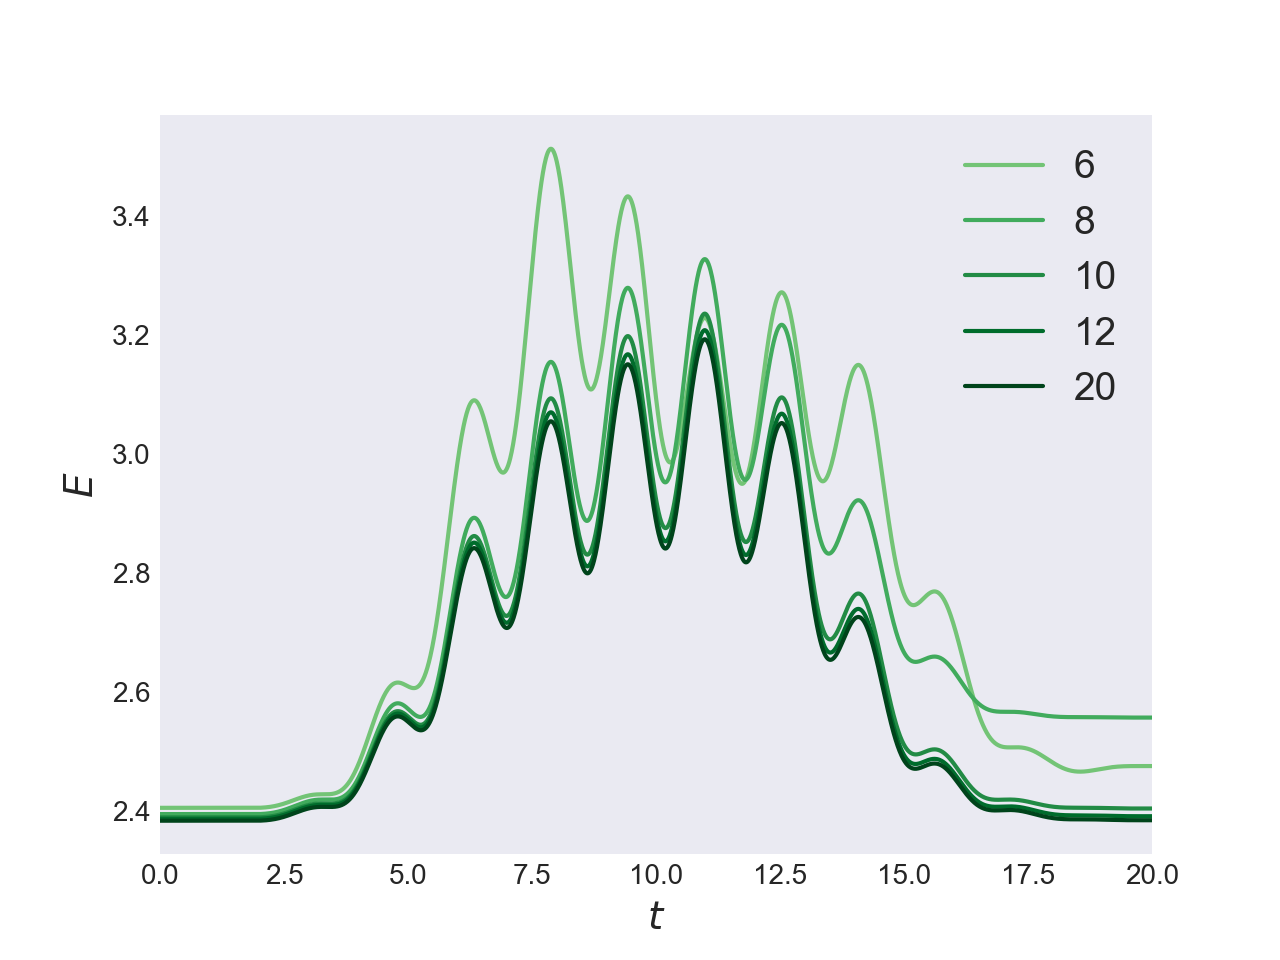
\includegraphics[width=0.75\textwidth]{results/figures/1D/n=2energy.png} 
    \caption{Time-dependent energy of a one-dimensional harmonic oscialltor 
        with $n=2$ electrons
        under the influence of a laser field for different number of spinorbitals
        $l\in\{6,8,10,12,20\}$.
    }
    \label{fig:1d_n2_E}
\end{figure}

First we study the time-dependent energy of a quantum dot acted upon by an oscillating 
field. The result for $n=2$ electrons is shown in \autoref{fig:1d_n2_E}. We have 
produced comparative results for other number of particles $n=\{4,6,8,10,12\}$,
which can be found in \autoref{app:1d_qd}. We see an apparent convergence in the 
time-dependent energy as we increase the number of spin-orbitals in the basis set.
For larger systems with more electrons it reasonably becomes necessary to also increase
the size of the basis set. As is the tendency with ground state coupled cluster computations
for quantum dots\cite{jorgensen2011many,lohne2010coupled}, the time dependent energy 
of a quantum dot is decreasing until convergence for increasing basis set size.

We see the same general convergent tendency when computing the time-dependent ground 
state probability $|\braket{\Psi(0)}{\Psi(t)}|^2$, shown in \autoref{fig:1d_n2_overlap} for $n=2$ electrons. We see that 
for lower number of spin-orbitals, the computation of overlap with 
the ground state tends to return a lower value than for a higher number of spin-orbitals.

\begin{figure}
    \centering
    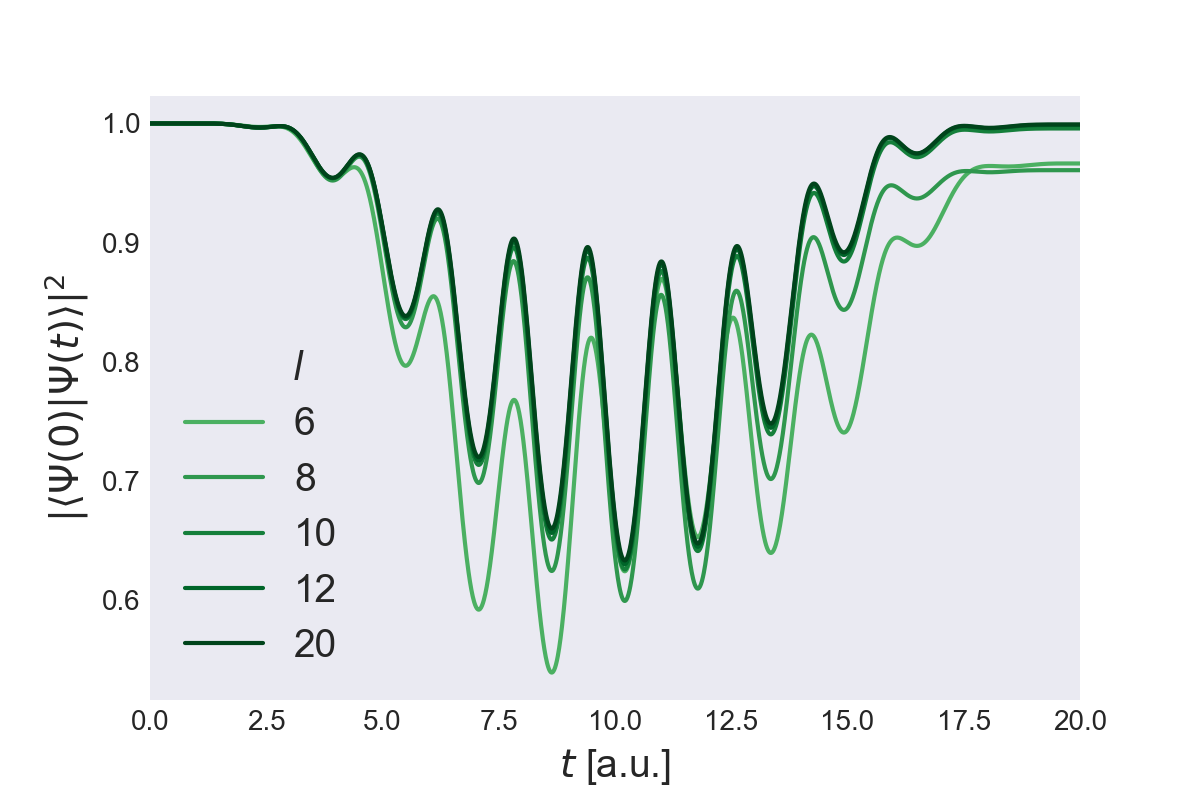
\includegraphics[width=0.75\textwidth]{results/figures/1D/n=2overlap.png} 
    \caption{Probability of being in the ground state $|\braket*{\Psi(0)}{\Psi(t)}|^2$
        for a one-dimensional quantum dot with $n=2$ electrons under 
        the influence of a laser field for different number of spinorbitals 
        $l\in\{6,8,10,12,20\}$.
    }
    \label{fig:1d_n2_overlap}
\end{figure}

Since the ground state probability is a number between zero and one, the results for systems 
of different number of electrons are comparable. We have produced such a comparison in 
\autoref{fig:1d_ground_state_prob_compare}. In this figure we have chosen the number of
spin-orbitals that would produce a convergent plot for the given system size. The general 
tendency is that a system with more electrons is less likely to be in the ground state 
over time, than a system with less electrons.

\begin{figure}
    \centering
    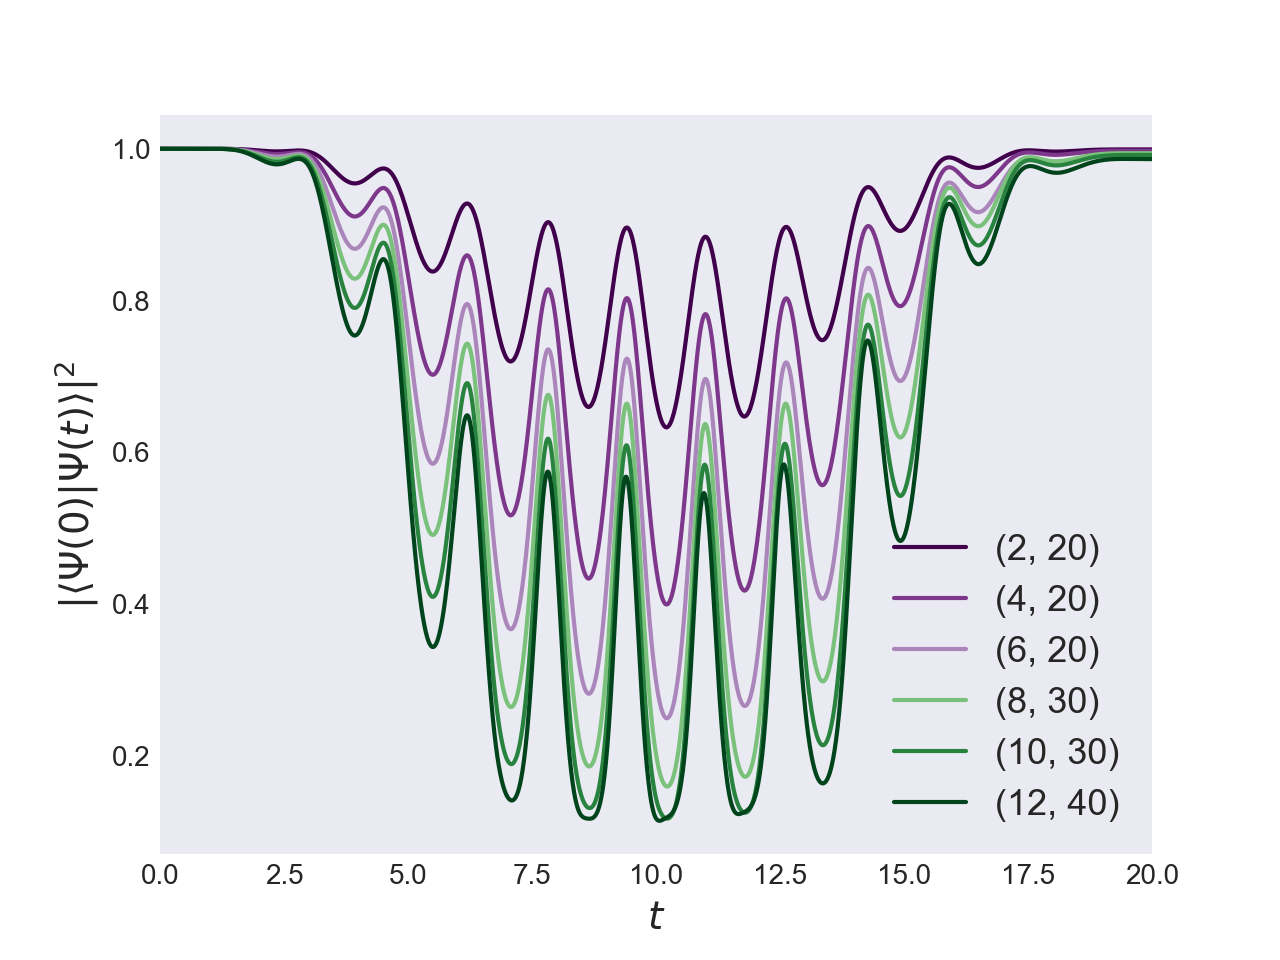
\includegraphics[width=0.75\textwidth]{results/figures/1D/n_compare_overlap.png} 
    \caption{Probability of being in the ground state for $|\braket*{\Psi(0)}{\Psi(t)}|^2$
        for a one-dimensional quantum dot for different number of electrons 
        $n\in\{2,4,6,8,10,12\}$.
    }
    \label{fig:1d_ground_state_prob_compare}
\end{figure}

\subsection{Dipole spectrum}

We now turn to a somewhat different kind of simulation. We keep the 
base system the same, a one-dimensional quantum dot with harmonic potential and oscillator 
frequency $\Omega=1$. We also apply an external oscillating field like in
\autoref{eq:results_1d_field}, which will this time be resonant with the frequency of the 
oscillator $\omega=\Omega=1$, to ensure population of excited states. In this simuation 
we set the field to zero at $T_d = 5 \text{ au}$, by the use of a Heaviside function in a 
similar manner as \citeauthor{pedersen2019symplectic}\cite{pedersen2019symplectic}
in \autoref{eq:pedersen_2019_envelope}. After the field has been switched off we propagate 
the system in time for a total of $T = 500 \text{ au}$ with a time step size of $dt=0.01$.
The same procedure is repeated for systems with $n=\{2,4,6,8,10,12\}$ electrons with 
respective number of spin-orbitals $l=\{20,20,20,30,30,40\}$. These system and basis 
sizes correspond to the ones used in \autoref{fig:1d_ground_state_prob_compare}.
For each time step we collect the dipole, i.e. $\ev{\hat{x}} = \tr{\rho x}$, and compute the 
Fourier transform of the entire collected array. The results are presented in 
\autoref{fig:1d_dipole_spectra}.

\begin{figure}
    \centering
    \makebox[\textwidth][c]{
    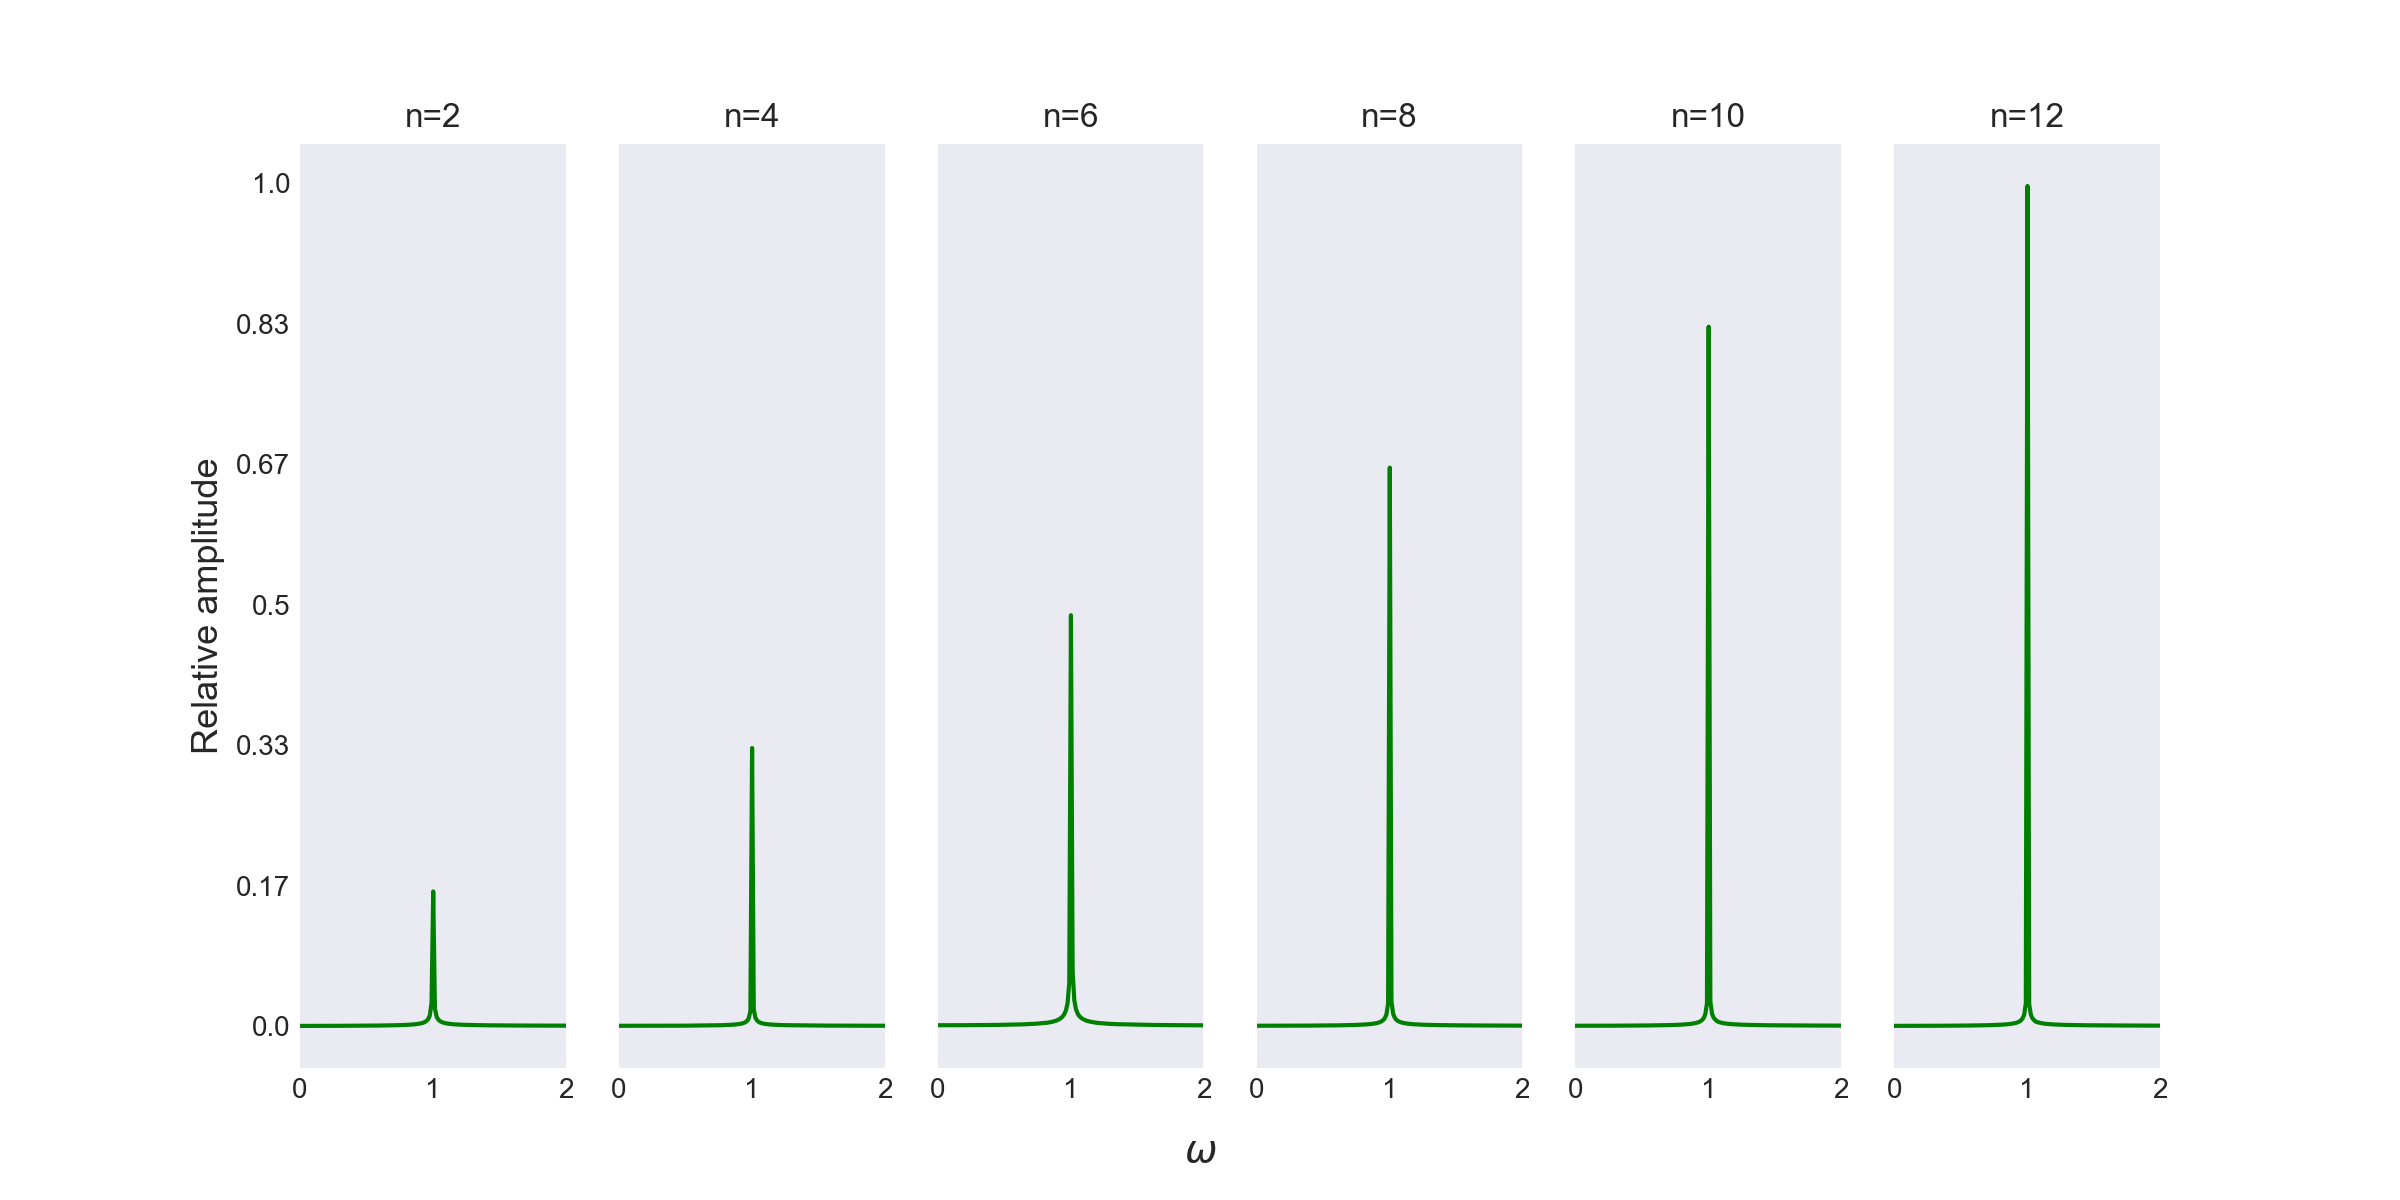
\includegraphics[width=1.4\textwidth]{results/figures/1D/1d_spectrum.png} 
    }
    \caption{Fourier transform of expected value of dipole moment for 
        a one-dimensional quantum dot with different number of electrons
        $n=\{2,4,6,8,10\}$ with respective number of spin-orbitals 
        $l=\{20,20,20,30,30,40\}$.
    }
    \label{fig:1d_dipole_spectra}
\end{figure}

We see that the result is in accordance with the harmonic potential theorem, as the 
simulations have produced dipole spectra that show only one line corresponding to the 
frequency of the confining potential. Morover, we see that the relative intensity of 
the spectra increases with the number of particles.

\subsection{Resonance Sensitivity}

In order to test the response of a quantum dot as the frequency of the oscillating 
field apporaches the oscillator frequency, we have run simulations for a selection 
of laser frequencies $\omega$ with the field described by \autoref{eq:results_1d_field}.
We chose frequencies $\omega\in\{1.0, 1.25, 1.5, 1.75, 2.0\}$ and set the 
oscillator freqcuencies of the quantum dot systems to $\Omega=1$. The laser pulse 
had a set period of $T_l=20 \text{ au}$, starting from $t=0$, while time-development 
of the system was allowed to continue to $T=30 \text{ au}$. The results of these 
simulations are shown for $n=2$ particles in \autoref{fig:n2_1d_resonance_energy}
and \autoref{fig:n2_1d_resonance_overlap}, which show the time-dependent energy 
and the time-dependendent ground state probabilities
$|\braket{\Psi(0)}{\Psi(t)}|^2$ respectively.

\begin{figure}
    \centering
    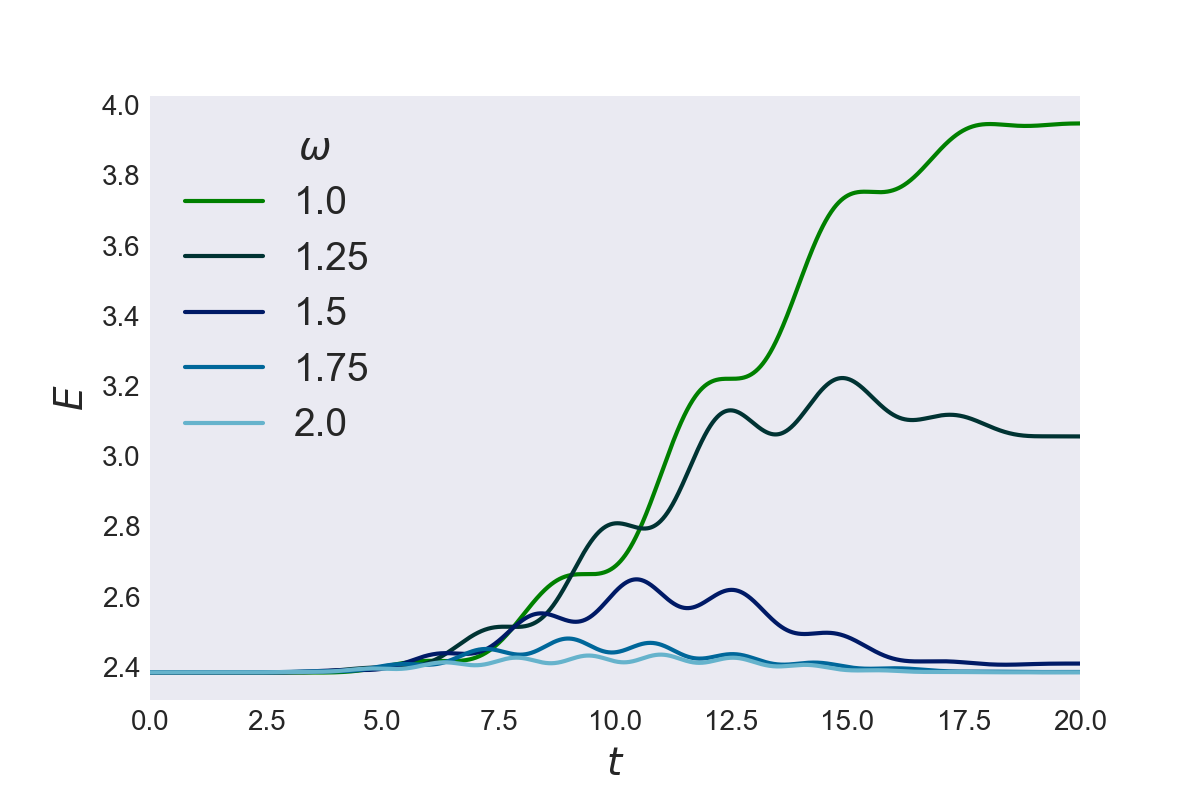
\includegraphics[width=0.75\textwidth]{results/figures/1D/n2_resonance_energy.png} 
    \caption{Time-dependent energy of a one-dimensional quantum dot with
        oscillator frequency $\Omega=1$ and $n=2$ electrons.
        The quantum dot is influenced by an oscillating field of different 
        frequencies $\omega\in\{1.0, 1.25, 1.5, 1.75, 2.0\}$ with a maximum 
        intensity of $\vb{E}_\text{max} = 0.25$.
    }
    \label{fig:n2_1d_resonance_energy}
\end{figure}

\begin{figure}
    \centering
    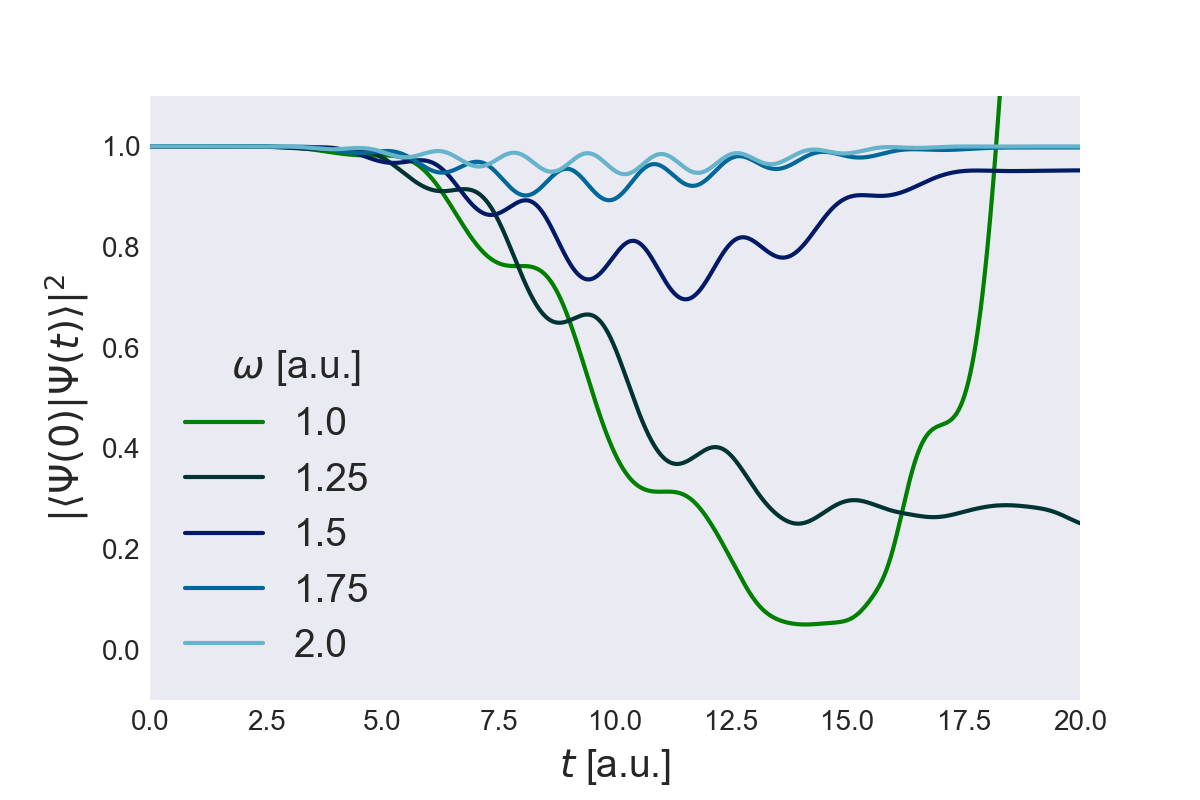
\includegraphics[width=0.75\textwidth]{results/figures/1D/n2_resonance_overlap.png} 
    \caption{Time-dependendent ground state probability $|\braket{\Psi(0)}{\Psi(t)}|^2$
        of a one-dimensional quantum dot with
        oscillator frequency $\Omega=1$ and $n=2$ electrons.
        The quantum dot is influenced by an oscillating field of different 
        frequencies $\omega\in\{1.0, 1.25, 1.5, 1.75, 2.0\}$ with a maximum 
        intensity of $\vb{E}_\text{max} = 0.25$.
    }
    \label{fig:n2_1d_resonance_overlap}
\end{figure}

The results are as expected, but interesting nonetheless. We see that the quantum dots 
behave very much as a classical driven harmonic oscillator. If the frequency of the driving
force, in this case the oscillating field, is far from the resonant frequency of the 
system the system falls back to the inital position after the force subsides. Only when we 
get closer to the resonant system do we see an excitation in energy of the system as 
a whole after the laser field is switched off (\autoref{fig:n2_1d_resonance_energy}).
In the case for the exact resonant frequency,
such that $\omega=\Omega$, we se that the energy of the system is increased even at the very 
end of the simulation, when the amplitude of the oscillating field is miniscule.
The same effects are apparent when studying the overlap of the time-developed system 
with the initial ground state in \autoref{fig:n2_1d_resonance_overlap}. Closer to the
resonant frequency we see a much lower probability of being in the ground state. For 
frequencies far away from the resonant frequency we see that the system falls back to 
the exact ground state or a state close to the ground state.

We have run similar simulations to the one described above, in order to study the 
resonant properties of a quantum dot, for $n=4,6,8,10$ electrons in a one-dimensional 
quantum dots. Figures with the results from these simulations can be found in 
\autoref{app:1d_qd}. In the ground state probability plots for these simulations, 
one would notice non-sensible probabiliy values $|\braket{\Psi(0)}{\Psi(t)}|^2 > 1$.
This is an issue we have adressed in the following sections, when reviewing the results 
of the two-dimensional quantum dot results.


\section{Two-dimensional Quantum Dot}

The two-dimensional quantum dot arguably paints a somewhat more interesting picture 
than the one-dimensional quantum dot, as we shall see. We construct several 
harmonic potential systems using the  \lstinline{TwoDimensionalharmonicOscillator}.
Similarly to the one-dimensional case, we simulate a laser by adding an 
oscillation field of the kind used by
\citeauthor{pedersen2019symplectic}\cite{pedersen2019symplectic}, shown 
in \autoref{eq:results_1d_field}. Because we have added a dimension, we must 
choose a direction of polarisation. This choice is arbitrary because of the 
symmertry of the quantum dots. We therefore arbitrarily pick the $x$-direction.
Unlike the one-dimensional dot, we are restricted to only a certan selection of 
systems, namely systems of $n\in\{2,6,12\}$ electrons, that ensure full shells.

Like in our simulations of a one-dimensional harmonic quantum dot we have at first 
sought to show that convergence in the computations by applying an oscillating 
field far from the resonant frequency of the system. We set the oscilaltor frequency 
to $\Omega=1$ and the frequency of the eletric field to $\omega=2\Omega=2$. We 
perform a simulation over a period $T = 20 \text{ au}$, for an increasing 
number of spin-orbitals $l$. The maximum intensity of the laser field is set to 
$\vb{E}_\text{max} = 1 \text{ au}$. For these initial computations we use the 
time-dependent coupled cluster singles doubles (TDCCSD) method with static 
orbitals. The simulations for two and six eletrons show expected results and have
therefore been consigned to \autoref{app:supp_2d_qd_results}, while the results for
twelve electrons appear to be on the brink of what the TDCCSD method 
can handle, within the given basis set size.

\begin{figure}
    \centering
    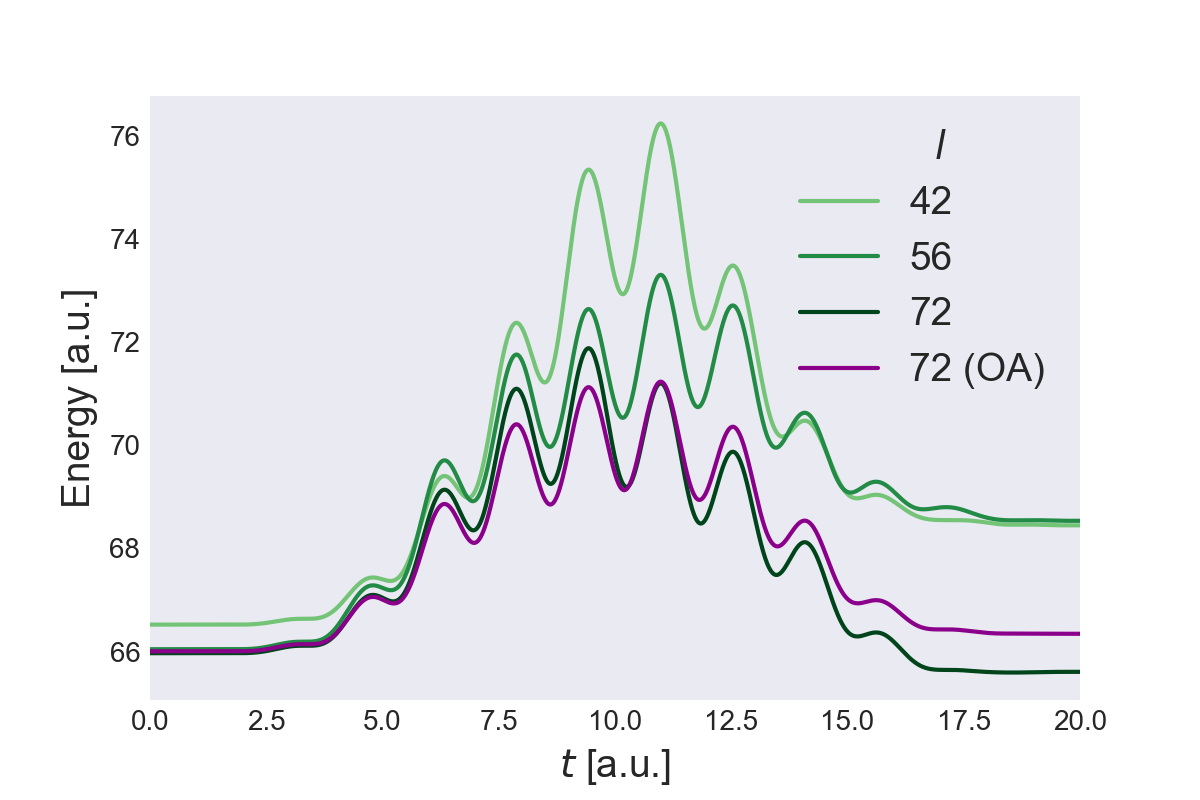
\includegraphics[width=0.75\textwidth]{results/figures/2D/n12_energy.png} 
    \caption{Time-dependent energy of a two-dimensional harmonic oscillator 
        with $n=12$ electrons under the influence of a laser field for different 
        spinorbitals $l\in\{42,56,72\}$.
    }
    \label{fig:n12_2d_energy}
\end{figure}

\begin{figure}
    \centering
    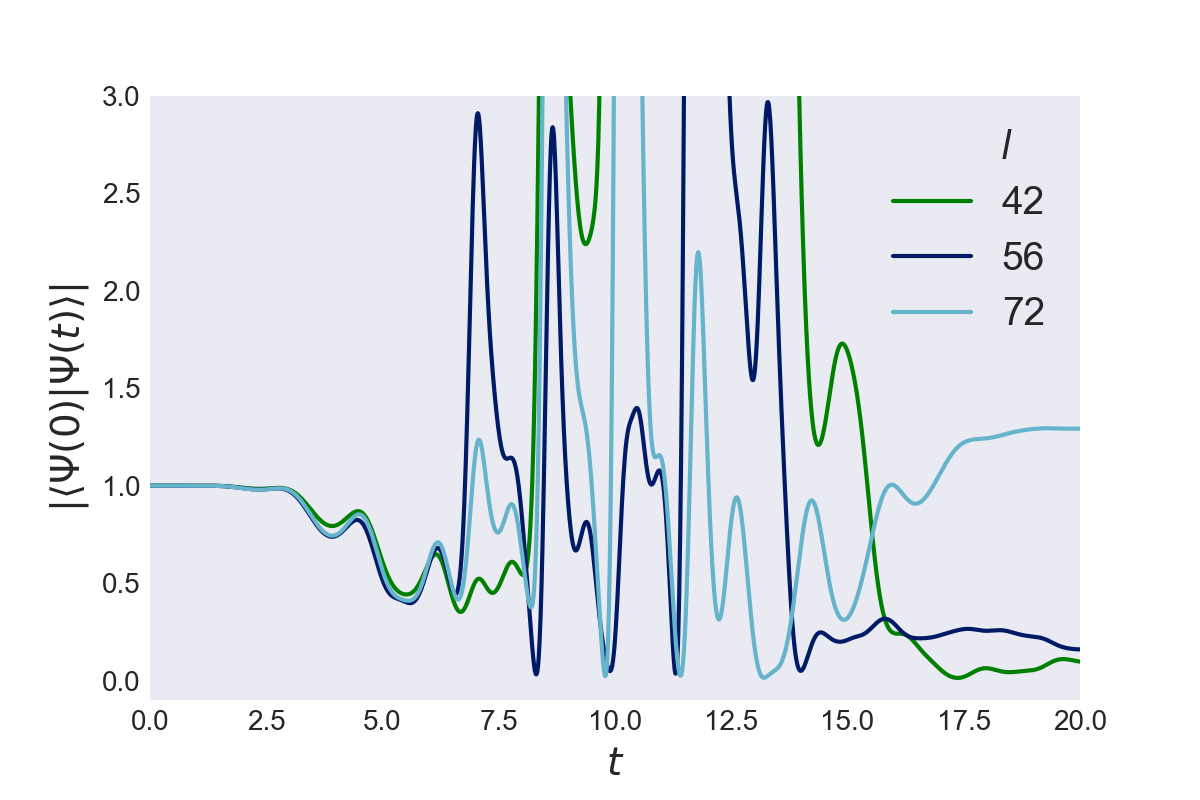
\includegraphics[width=0.75\textwidth]{results/figures/2D/n12_overlap.png} 
    \caption{Ground state probability $|\braket{\Psi(0)}{\Psi(t)}|^2$ for two-dimensional
        quantum dot with $n=12$ electrons under the influence of a laser field for 
        different number of spinorbitals $l=\{42,56,72\}$. 
    }
    \label{fig:n12_2d_overlap}
\end{figure}

The time-dependent energy of a two-dimensional harmonic quantum dot with $n=12$
electrons under influence of the oscillating field described above is shown in 
\autoref{fig:n12_2d_energy}. In this figure we have run the same simulation for 
$l\in\{42,56,72\}$ spin-orbitals with the time-dependent coupled cluster 
singles doubles (TDCCSD) method, and we see that only for the very largest of the 
basis set to we see a behaviour conforming with our expectations. We expect the 
energy to be close to the ground state energy after the laser-field has died down.

In the same figure (\autoref{fig:n12_2d_energy}) we have also included
the computed energy over time for the system using the
orbital-adaptive time-dependent coupled cluster doubles (OATDCCD) method and the 
same number if spin-orbitals.
We see that the two methods dont't agree completely, and we are prone to trust 
the OATDCCSD method more than the TDCCSD method in this case, because the energy at 
the end of the simulations is lower than the initial energy for the TDCCSD method.
The reason for the problems the TDCCSD method shows are likely caused by our attempt 
to represent a state with the basis functions contained in the reference,
which is very dissimilar to said reference function. We will outline this problem 
further as we study the time-dependent ground state probability of the simulation.

The ground state probability of the same simulation with the TDDCCSD method 
is shown in
\autoref{fig:n12_2d_overlap}. We see immediately that the probability becomes 
non-sensical at some time step after $t=6 \text{ au}$. This result is similar to
the sort of break-down that occured for the TDCCSD method in the attempt to 
replicate the results of \citeauthor{miyagi2013time}\cite{miyagi2013time} in
\autoref{sec:miyagi_replication}.

The probable cause of the non-sensible 
ground state probability is the need for the amplitudes of the system to acquire 
relatively high values, in order to compensate for the inadequateness of the 
reference state to describe the exact time-dependent state. This is underlined 
by the norm of the amplitudes, displayed in \autoref{fig:n12_2d_amp_norms}. As 
is apparent, the lambda amplitudes shows an upwards trend throughout the 
simulation.
This should be unnecessary because the system would revert back to a state 
similar to the ground state at the end of the simulation. It appears that 
some ``tipping point'' is reached halfway around $t=T/2$ when instabillty 
increases. The tau amplitudes are more or less well-behaved, at least for 
the largest basis set, showing some correlation in amplitude with the
sinusoidal envelope of the oscillating field.

\begin{figure}
    \centering
    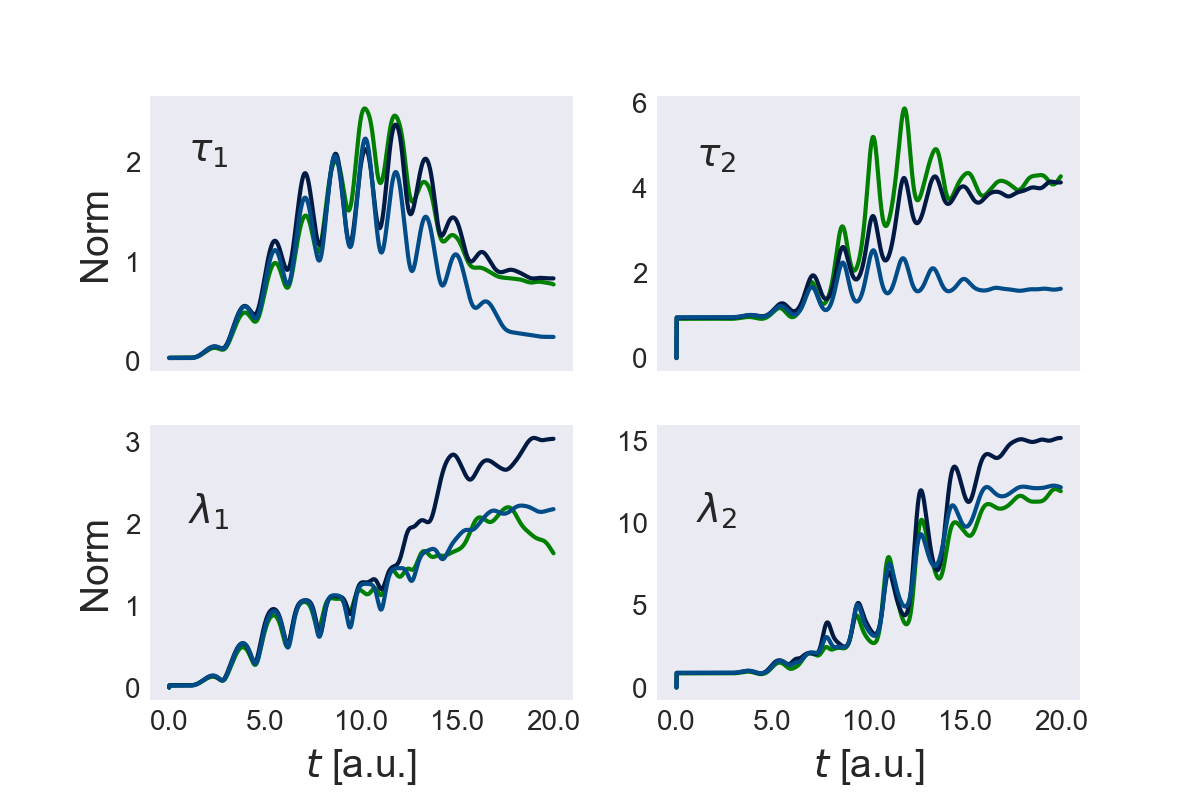
\includegraphics[width=0.9\textwidth]{results/figures/2D/n=12_amplitudes.png}
    \caption{Norm of amplitudes in a $n=12$ electron two-dimensional quantum 
        dot influenced by an oscilalting field, for several number of 
        spin-orbitals $l=\{42,56,72\}$.
    }
    \label{fig:n12_2d_amp_norms}
\end{figure}

\subsection{Dipole Spectrum}

We have for the two-dimensional quantum dot computed dipole spectrum for systems of 
different size, like we did fro the one-dimensiaonal quantum dot. We did this for 
quantum dots with oscillator frequencies $\Omega=1$ with $n\in\{2,6,12\}$ electrons.
We used $l\in\{42,42,56\}$ as the number of spinorbitals for the respective systems.
In order to excite and disturb the systems from the inial ground state we applied 
an oscillating field with a resonant frequency $\omega=\Omega=1$ and a somewhat low 
maximum intensity $\vb{E}_\text{max}=0.1$, with a three-step linear envelope as 
in \autoref{eq:li_laser}. The systems were allowed to develop in time for 
$T = 500 \text{ au}$. The results of computing the Fourier transform of the 
dipole $\vb{x} = \tr{\rho x}$ is depicted in \autoref{fig:2d_dipole_spectra}. 
In this figure we see that the result is qualtitatively in accordance with the 
harmonic potential theorem - the dipole freqcuencies of all the systems are the 
same, with an intensity that increases with the number of particles in the system.
For the two larger systems with $n=6$ and $n=12$ electrons we see some slight 
inccuracies. These are attributable to the time constraint of this study - 
a simulation with larger number of spinorbitals would have remedies these 
inaccuracies, but would have needed more time to complete.

\begin{figure}
    \centering
    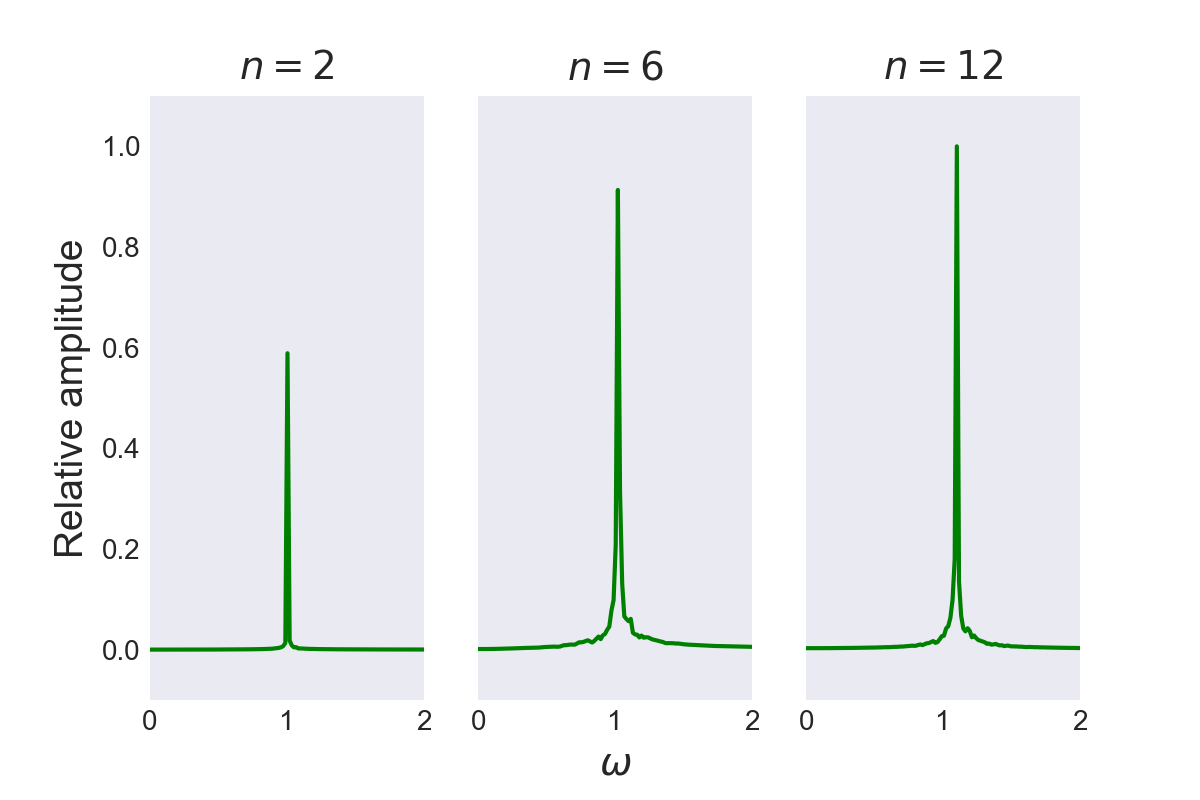
\includegraphics[width=0.9\textwidth]{results/figures/2D/2d_spectrum.png} 
    \caption{Fourier transform of expected value of dipole moment for a
        two-dimensional quantum dot with different number of electrons 
        $n=\{2,6,12\}$ and respective number of spin-orbitals 
        $l=\{40,40,56\}$.
    }
    \label{fig:2d_dipole_spectra}
\end{figure}

\subsection{Resonance Sensitivity}

For the two-dimensiona quantum dot we have also conducted a resonance sensitivity analysis,
similar to the one we performed for the one-dimensional quantum dot. The results for 
$n=2$ electrons and $n=6$ electrons are displayed in \autoref{fig:2d_resonance_n2}
and \autoref{fig:2d_resonance_n6} respectively. The quantum dots in these simualtions 
had an oscillator frequency of $\Omega=1$ and where subjected to an oscillating 
field with a sinusoidal envelope of the type in \autoref{eq:results_1d_field} of 
different frequencies $\omega\in\{1.0,1.25,1.5,1.75,2.0\}$ and a maximum intensity of 
$\vb{E}_\text{max}=0.25$. The simulations were done with the time-dependent coupled 
cluster doubles (TDCCSD) method with static orbitals.

Like in the one-dimensional analysis we see that the systems are much more prone to 
excitation as the frequency of the laser field approaches that of the quantum harmonic 
oscillator. This is apparent both for the energy of the quantum dot systems and the 
ground state probabilites displayed in the left and right subfigures of
\autoref{fig:2d_resonance_n2} and \autoref{fig:2d_resonance_n6}, respectively. In the 
six-particle case we again see the problems with the TDCCSD method when computing the 
ground state overlap, as the amplitudes acquire higher and higher values, resulting 
in non-sensical probability values. However, in this case we do belive that the 
energy plots to be qualitatively correct.

\begin{figure}
    \centering
    \begin{minipage}{0.49\textwidth}
        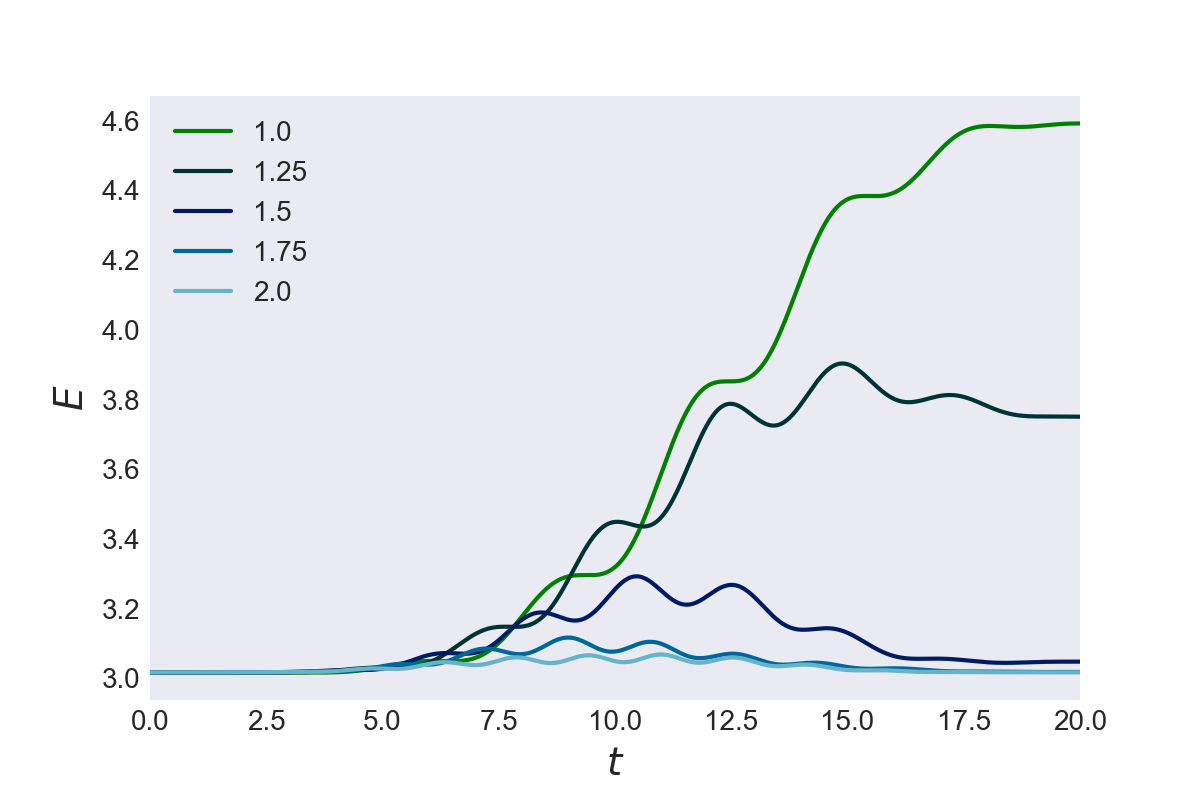
\includegraphics[trim=2em 0em 5em 0em, width=\textwidth]{results/figures/2D/resonance/n2resonance.png} 
    \end{minipage}\hfill
    \begin{minipage}{0.49\textwidth}
        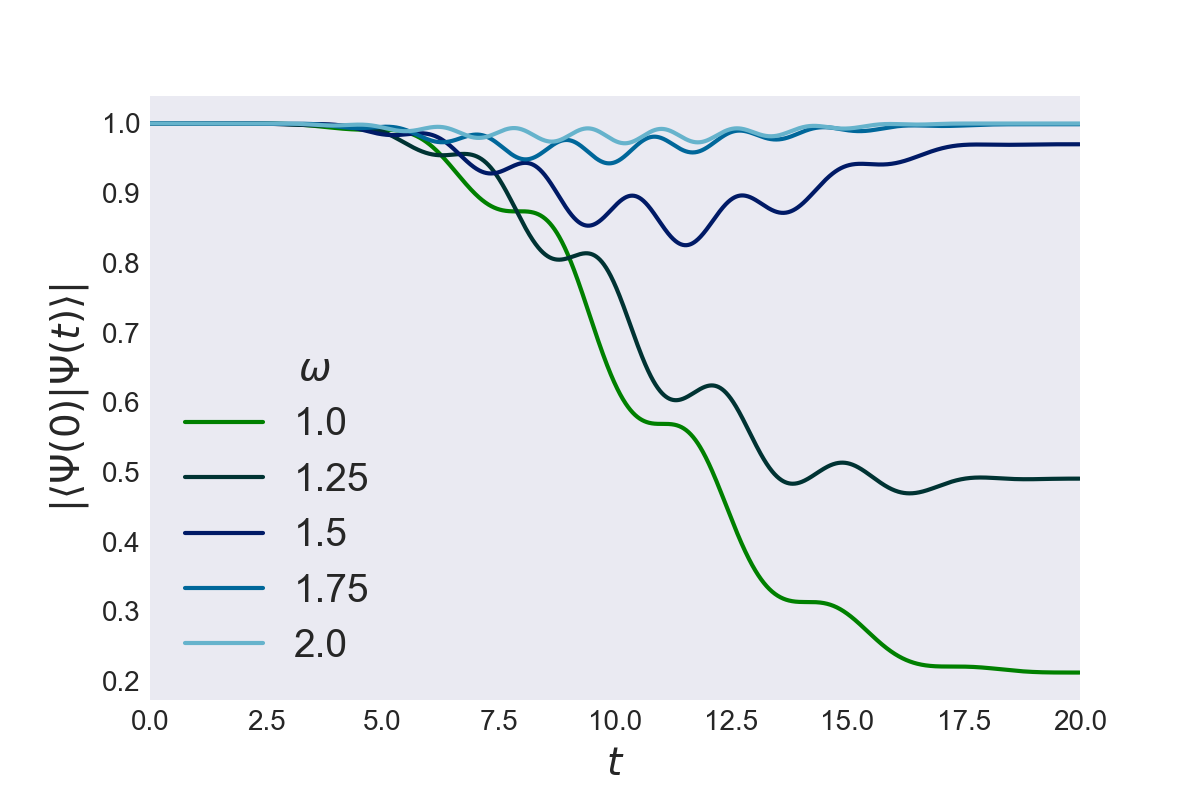
\includegraphics[trim=0em 0em 5em 0em, width=\textwidth]{results/figures/2D/resonance/n2overlap_res.png} 
    \end{minipage}
    \caption{Time dependent energy (left) and ground state probability $|\braket{\Psi(0)}{\Psi(t)}|^2$
        (right) for a two-dimensional quantum dot with $n=2$ electrons. The quantum dot 
        is affected by an oscillating field of different frequencies
        $\omega\in\{1.0, 1.25, 1.5, 1.75, 2.0\}$ with a maximum inntensity
        $\vb{E}_\text{max} = 0.25$. The confining harmonic potential has frequency $\Omega=1$.
    }
    \label{fig:2d_resonance_n2}
\end{figure}

\begin{figure}
    \centering
    \begin{minipage}{0.49\textwidth}
        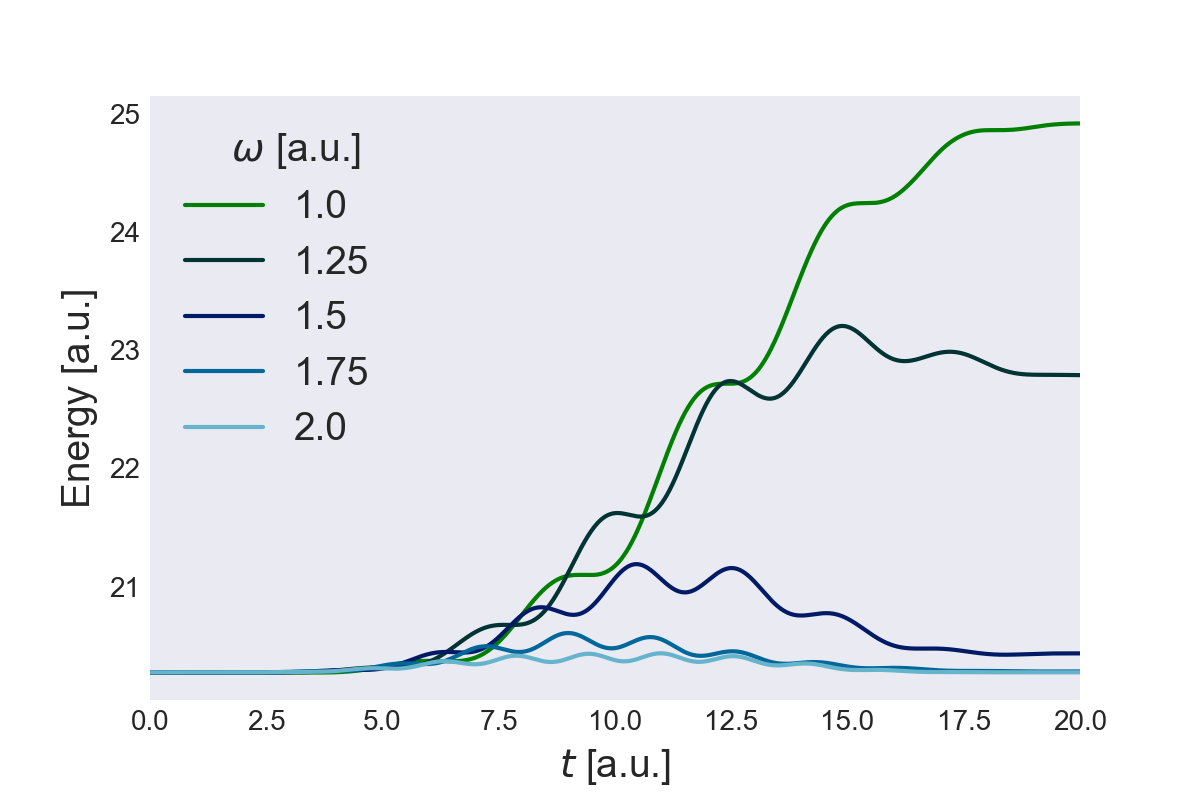
\includegraphics[trim=2em 0em 5em 0em, width=\textwidth]{results/figures/2D/resonance/n6resonance.png} 
    \end{minipage}\hfill
    \begin{minipage}{0.49\textwidth}
        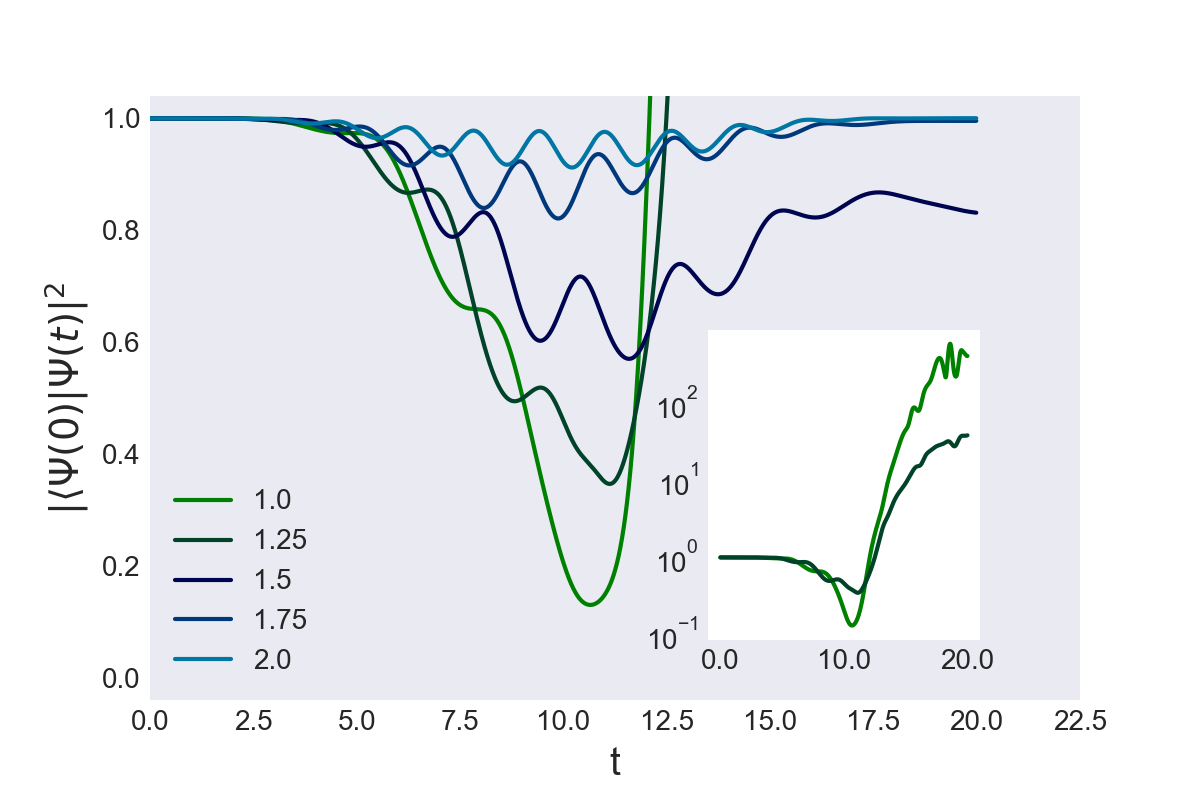
\includegraphics[trim=0em 0em 5em 0em, width=\textwidth]{results/figures/2D/resonance/n6_overlap_res.png} 
    \end{minipage}
    \caption{Time dependent energy (left) and ground state probability $|\braket{\Psi(0)}{\Psi(t)}|^2$
        (right) for a two-dimensional quantum dot with $n=6$ electrons. The quantum dot 
        is affected by an oscillating field of different frequencies
        $\omega\in\{1.0, 1.25, 1.5, 1.75, 2.0\}$ with a maximum inntensity
        $\vb{E}_\text{max} = 0.25$. The confining harmonic potential has frequency $\Omega=1$.
    }
    \label{fig:2d_resonance_n6}
\end{figure}


\section{Two-dimensional Double Dot}

We have simulated two different two-dimensional double dot systems, one with $n=2$ electrons 
and 
one system with $n=4$ electrons, using the \lstinline{TwoDimensionalDoubleWell} class described
in \autoref{sec:2d_double_well}. We use $l=20$ spin-orbitals for the two-electron system 
and $l=56$ spin-orbitals for the four-electron system. The class requires two special parameters, 
\lstinline{l_ho_factor} and \lstinline{barrier_strength}, that define the 
number of regular harmonic oscillator functions to map to and the height of the 
barrier in the middle of the well, respectively. We set the barrier strength to $2$ 
and the harmonic oscillator factor to $2$ for both systems. The oscillator frequency 
of the double dot is set to $\Omega=1$. As a visual confirmation of the systems, a 
one-electron density plot is provided for the $n=2$ electrons system (left) and 
the $n=4$ electron system (right) in \autoref{fig:2d_dw_rho}.

The double dot is in essence a perturbation of the regular two-dimensional quantum dot, and we are seeking to uncover any many-body 
effects that such a perturbation could lead to. In order to do this we would like to 
compute the dipole spectrum of both systems. The time-propagation is done using the 
orbital-adaptive time-dependent coupled cluster doubles (OATDCCD) method, as it has shown 
the best stability of our time-dependent methods. Both systems are under the influence of an 
oscillating field with a linearly decreasing- and increasing envelope of the type used by 
\citeauthor{li2005time}\cite{li2005time} (\autoref{fig:li_compare}). We have chosen a 
frequency of this field that corresponds to the resonant of the first transition energy 
of the system $\omega = 0.43 \text{ au}$, and an intensity yielding a maximum amplitude
$\vb{E}_\text{max} = 0.1 \text{ au}$. The resonant frequency was found by direct diagonalisation 
of the one-body matrix produced by the system class \lstinline{TwoDimensionalDoubleWell}.

\begin{figure}
    \centering
    \begin{minipage}{0.49\textwidth}
        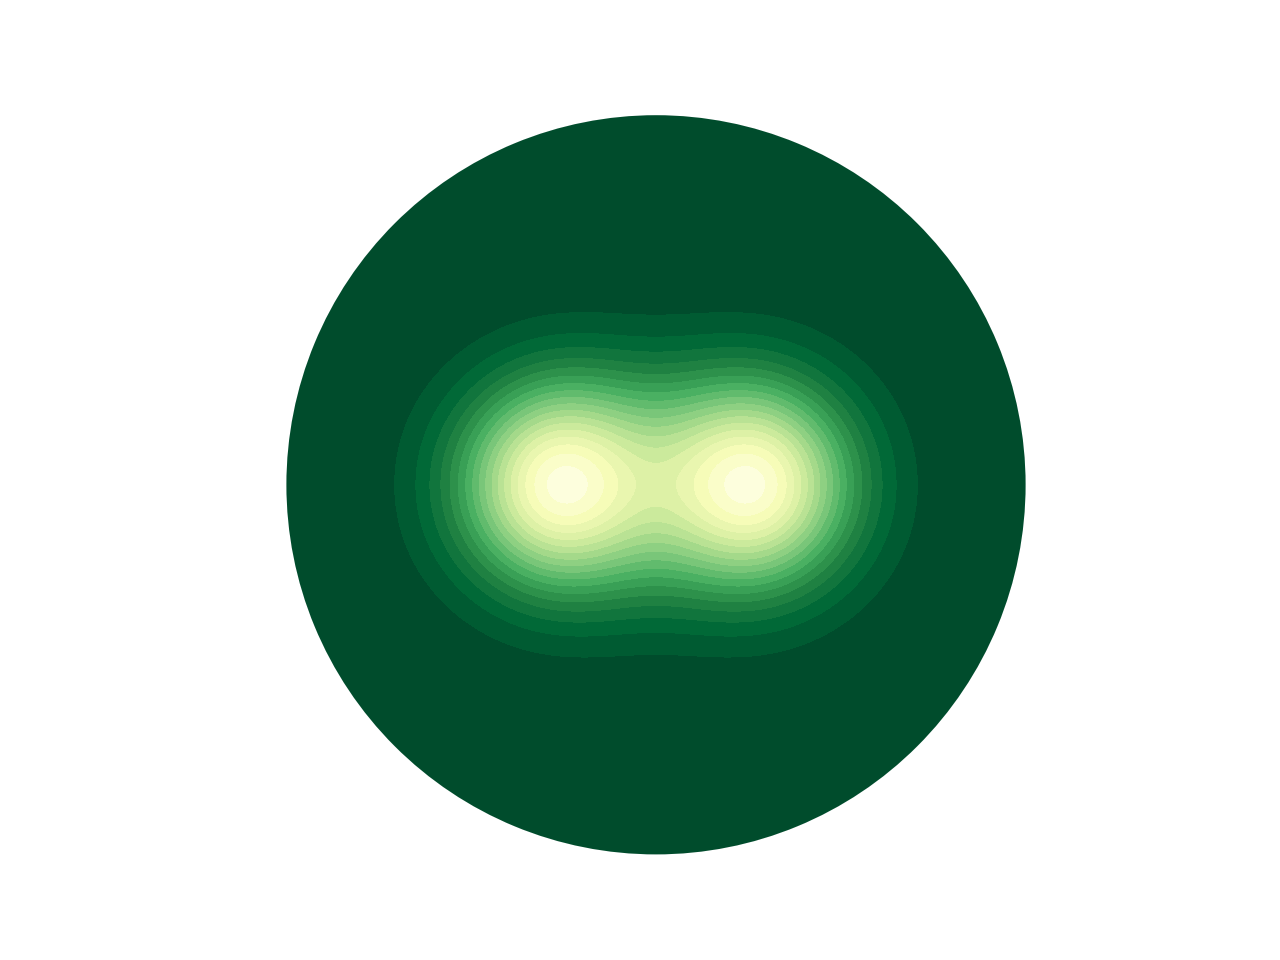
\includegraphics[trim=4em 3.5em 4em 4em, clip=true, width=\textwidth]{results/figures/DW/rho_dw.png} 
    \end{minipage}\hfill
    \begin{minipage}{0.49\textwidth}
        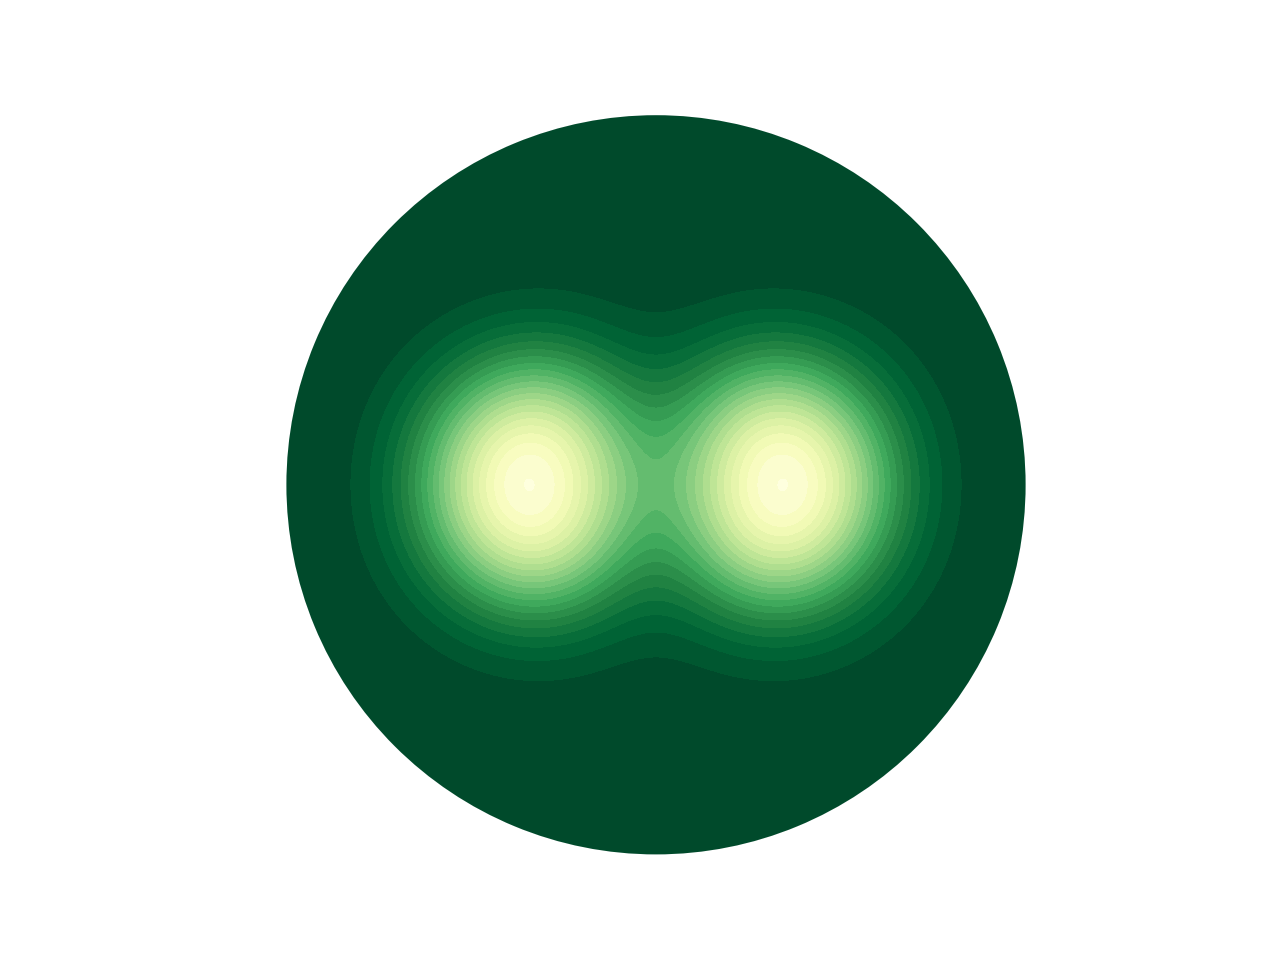
\includegraphics[trim=4em 3.5em 4em 4em, clip=true, width=\textwidth]{results/figures/DW/rho_dw_n4.png} 
    \end{minipage}
    \caption{Ground state one-electron density for $n=2$ electrons (left)
        and $n=4$ electrons (right) for a double quantum dot.
    }
    \label{fig:2d_dw_rho}
\end{figure}

\begin{figure}
    \centering
    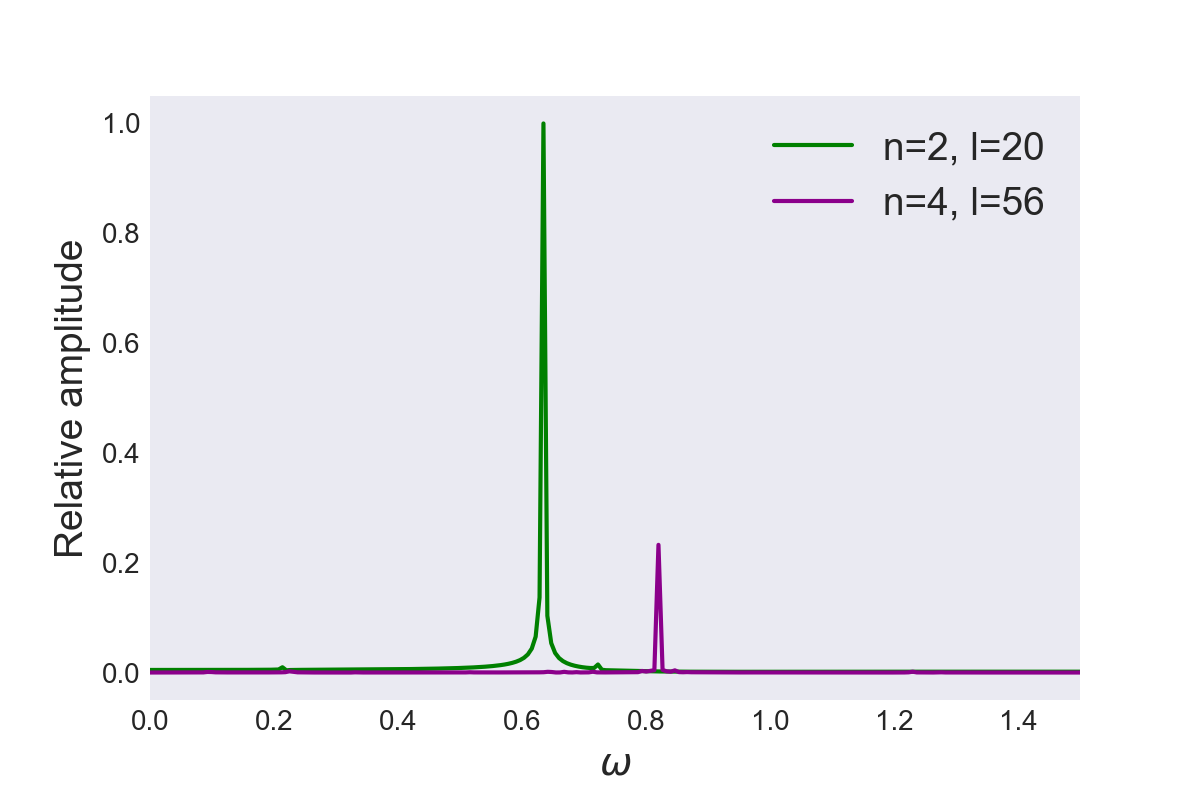
\includegraphics[width=0.75\textwidth]{results/figures/DW/dw_n2_n4_spectrum.png} 
    \caption{Dipole spectrum of two-dimensional double dot system with $n\in\{2,4\}$
        electrons and $l\in\{20, 56\}$ spinorbitals. 
    }
    \label{fig:2d_dw_n2_n4_spectra}
\end{figure}

The system is allowed to develop in time for $T = 100 \hat{ au}$ and complute the Fourier 
transform of the dipole moment $\ev{x} = \tr{\rho x}$, the results of which are shown 
in \autoref{fig:2d_dw_n2_n4_spectra}. We immediately see that there is only one frequency 
apparent in the spectra for each of the systems, meaning that the quantum double dots
have a position operators that behaves as if it was the centre of mass of the system. We 
see that the larger system has a somewhat more rapid movement relative to the smaller 
system. We also see that the larger system has lower intensity compared with the smaller 
system. This mya be because there is relatively more mass in the system to move, and the 
intensity of the laser field is unchanged.

\section{Two-dimensional Magnetic Quantum Dot}

We start the study of two-dimensional quantum dots under the influence of a magnetic 
field by defining a system of only one particle and solving the time-dependent 
Schrödinger equation
directly. This is a accomplished by using the \lstinline{TwoDimHarmonicOscB} class
to produce a basis set, single-particle functions and transition/intearction matrix (dipole elements),
which is everything we need. All of these items are properties of the class and can be
easily extracted. A simple periodic function simulates an electric field is constructed, as 
the product of such a time-dependent operator and the interaction matrix defines the 
time propagation. We then use a simple integration scheme, in this case the fourth-order 
Runge-Kutta method, to propagate the ground state single particle function of the system.
Taking care to extract the dipole for every time step, we can compute the discrete Fourier 
transform of the dipole and compute the frequency spectrum of our system. This procedure is 
applied to a system comletely absent of a magnetic field, and a system under direct influence 
of a magnetic field.

Before going straight to the results, we study the shell structure and allowed transitions of 
our two systems. The left part of \autoref{fig:shell_structure_yes_no_b} presents the 
shell structure of a the regular two-dimensional quantum dot. The states have all been assigned
a number for easier examination. This shell structure is 
identical to the one presented in \autoref{fig:2d_basis_states}. Additionally, here we have added
coloured double arrows to illustrate the allowed transitions in the quantum dot. These 
transitions are can be encountered in the transition matrix for the system, which is
reproduced in the artistic way in \autoref{fig:transition_no_b}. Notice that the coloured 
arrows representing allowed transitions match in colour with the elements of the transition 
matrix.

\begin{figure}
    \begin{center}
    \begin{tikzpicture}[scale=0.9, background rectangle/.style={fill=grey},
        show background rectangle]
    \begin{scope}
      
        % TOP
        \foreach \i in {0, 3, 6} {
            \draw(\i, 2) -- (\i + 2, 2);
            \node at (\i + 0.75, 2) {$\uparrow$};
            \node at (\i + 1.25, 2) {$\downarrow$};
        }
       
        \node[below, inner sep=.5em] at (1, 2) {$(0, -2)$};
        \node[above] at (1, 2) {5};
        \node[below, inner sep=.5em] at (4, 2) {$(1, 0)$};
        \node[above] at (4, 2) {3};
        \node[below, inner sep=.5em] at (7, 2) {$(0, 2)$};
        \node[above] at (7, 2) {4};

        % MIDDLE
        \foreach \i in {1.5, 4.5} {
            \draw(\i, 1) -- (\i + 2, 1);
            \node at (\i + 0.75, 1) {$\uparrow$};
            \node at (\i + 1.25, 1) {$\downarrow$};
        }

        \node[below, inner sep=.5em] at (2.5, 1) {$(0, -1)$};
        \node[above] at (2.5, 1) {1};
        \node[below, inner sep=.5em] at (5.5, 1) {$(0, 1)$};
        \node[above] at (5.5, 1) {2};

        % BOTTOM
        \draw(3, 0) -- (5, 0);
        \node at (3 + 0.75, 0) {$\uparrow$};
        \node at (3 + 1.25, 0) {$\downarrow$};

        \node[below, inner sep=.5em] at (4, 0) {$(0, 0)$};
        \node[above] at (4, 0) {0};

        % Transitions
        \draw [<->, line width=.1em, transition11] (3.5, 0) -- (3.25, 1);
        \draw [<->, line width=.1em, transition11] (4.5, 0) -- (4.75, 1);

        \draw [<->, line width=.1em, transition12] (3, 1) -- (3.25, 2);
        \draw [<->, line width=.1em, transition12] (5, 1) -- (4.75, 2);

        \draw [<->, line width=.1em, transition13] (2, 1) -- (1.75, 2);
        \draw [<->, line width=.1em, transition13] (6, 1) -- (6.25, 2);

    \end{scope}

    \begin{scope}[xshift=20em]

        % MIDDLE 2
        \foreach \i in {1.5, 4.5} {
            \draw(\i, 3) -- (\i + 2, 3);
            \node at (\i + 0.75, 3) {$\uparrow$};
            \node at (\i + 1.25, 3) {$\downarrow$};
        }

        \node[below, inner sep=.5em] at (2.5, 3) {$(1, 0)$};
        \node[above] at (2.5, 3) {3};
        \node[below, inner sep=.5em] at (5.5, 3) {$(0, 3)$};
        \node[above] at (5.5, 3) {6};

        % MIDDLE 1
        \foreach \i in {1.5, 4.5} {
            \draw(\i, 2) -- (\i + 2, 2);
            \node at (\i + 0.75, 2) {$\uparrow$};
            \node at (\i + 1.25, 2) {$\downarrow$};
        }

        \node[below, inner sep=.5em] at (2.5, 2) {$(0, -1)$};
        \node[above] at (2.5, 2) {1};
        \node[below, inner sep=.5em] at (5.5, 2) {$(0, 2)$};
        \node[above] at (5.5, 2) {4};

        % BOTTOM 2
        \draw(3, 1) -- (5, 1);
        \node at (3 + 0.75, 1) {$\uparrow$};
        \node at (3 + 1.25, 1) {$\downarrow$};

        \node[below, inner sep=.5em] at (4, 1) {$(0, 1)$};
        \node[above] at (4, 1) {2};
        
        % BOTTOM 1
        \draw(3, 0) -- (5, 0);
        \node at (3 + 0.75, 0) {$\uparrow$};
        \node at (3 + 1.25, 0) {$\downarrow$};

        \node[below, inner sep=.5em] at (4, 0) {$(0, 0)$};
        \node[above] at (4, 0) {0};
        
        % Transitions 

        % 0 -> 1
        \draw [<->, line width=.1em, transition21] (3.5, 0) to[out=120, in=-90] (1.75, 2);
        % 0 -> 2
        \draw [<->, line width=.1em, transition21] (4.5, 0) -- (4.5, 1);

        % 2 -> 3
        \draw [<->, line width=.1em, transition23] (3.5, 1) to[out=60, in=-50] (3.25, 3);
        % 2 -> 4
        \draw [<->, line width=.1em, transition22] (4.75, 1) -- (4.75, 2);

        % 1 -> 3
        \draw [<->, line width=.1em, transition23] (2, 2) -- (2, 3);
        % 4 -> 6 
        \draw [<->, line width=.1em, transition24] (6, 2) -- (6, 3);

    \end{scope}
    \end{tikzpicture}
    \end{center} 
    \caption{Shell structure of six lowest orbitals before (left), and after (right)
        a magnetic field is applied to a 2D quantum dot.}
    \label{fig:shell_structure_yes_no_b}
\end{figure}

When we apply apply a magnetic field of strength $\omega_c/\omega = \sqrt{2}/2$ we 
obtain the shell structure represented to the right in 
\autoref{fig:shell_structure_yes_no_b}, where the allowed transitions correpsond to the 
transition matrix in \autoref{fig:transition_yes_b}. The chosen magnetic field strength 
was not chosen arbitrarily, as these accidental degenracies occur only rarely as 
a function of magnetic field strength\footnote{Hence the term ``accidental''.}.
For succinctness we repeat the function for energy eigenvalues for two-dimensional 
quantum dot influenced by a magnetic field (\autoref{eq:2d_b_eigenvalues}),
\begin{equation}
    \epsilon_{nm} = \hbar\Omega(2n + |m| + 1) - \frac{\hbar\omega_c}{2}m,
\end{equation}
where $\Omega = \sqrt{\omega_0^2 + \frac{\omega_c^2}{4}}$.
Apart from a general shift up in energy by adding a magnetic field, the states with 
negative azimuthal quantum number $m$ will experience an increase in energy eigenvalue,
and vice versa. We see this effect clearly in the new shell structure in
\autoref{fig:shell_structure_yes_no_b}. The states with negative $m$ have indeed
undergone a relative shift upwards, whilst the states with positive $m$ have been
shifted downwards, relative to the other states. The ground state, labelled 0, 
remains relatively stationary, the states labelled 2 ($m=1$) and 4 ($m=2$) have been 
shifted downwards and the states labelled 1 ($m=-1$) and 5 ($m=-2$) have been shifted 
upwards. State number 5 so much that it has disappeared from the shell structure, with a 
new state 6 ($=3$) appearing. This is due to our restriction to include only the six
lowest-energy orbitals. We see that the possible remaining allowed transitions remain the 
same, with the exception of transitioning between state 1 and 5, because state 5 is no more,
and the addition of a possible transition between state 4 and 6.

\begin{figure}
    \begin{center}
    \begin{minipage}{0.49\textwidth}
        \centering
        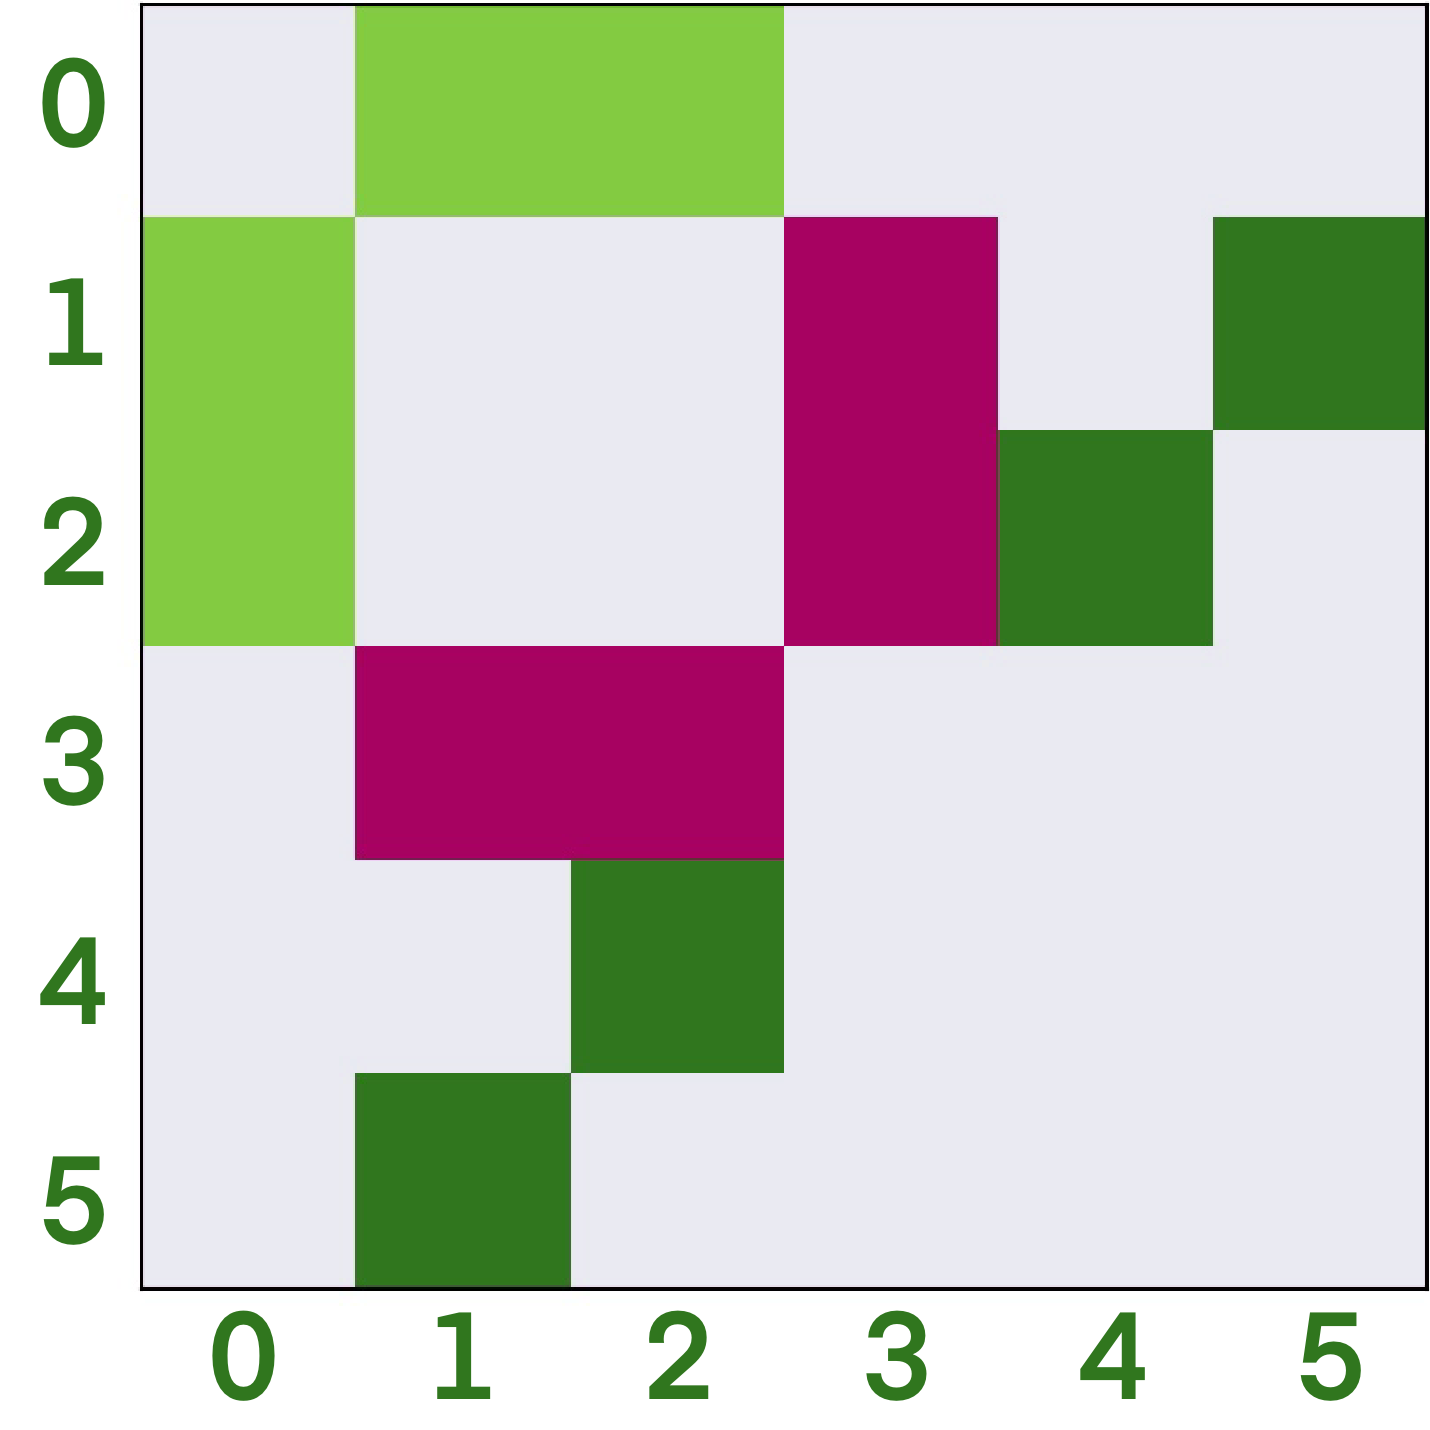
\includegraphics[width=\textwidth]{results/figures/dipole_no_b.png}
        \caption{Transition matrix dictating the allowed transitions for a
            2D quantum dot.}
        \label{fig:transition_no_b}
    \end{minipage}
    \begin{minipage}{0.49\textwidth}
        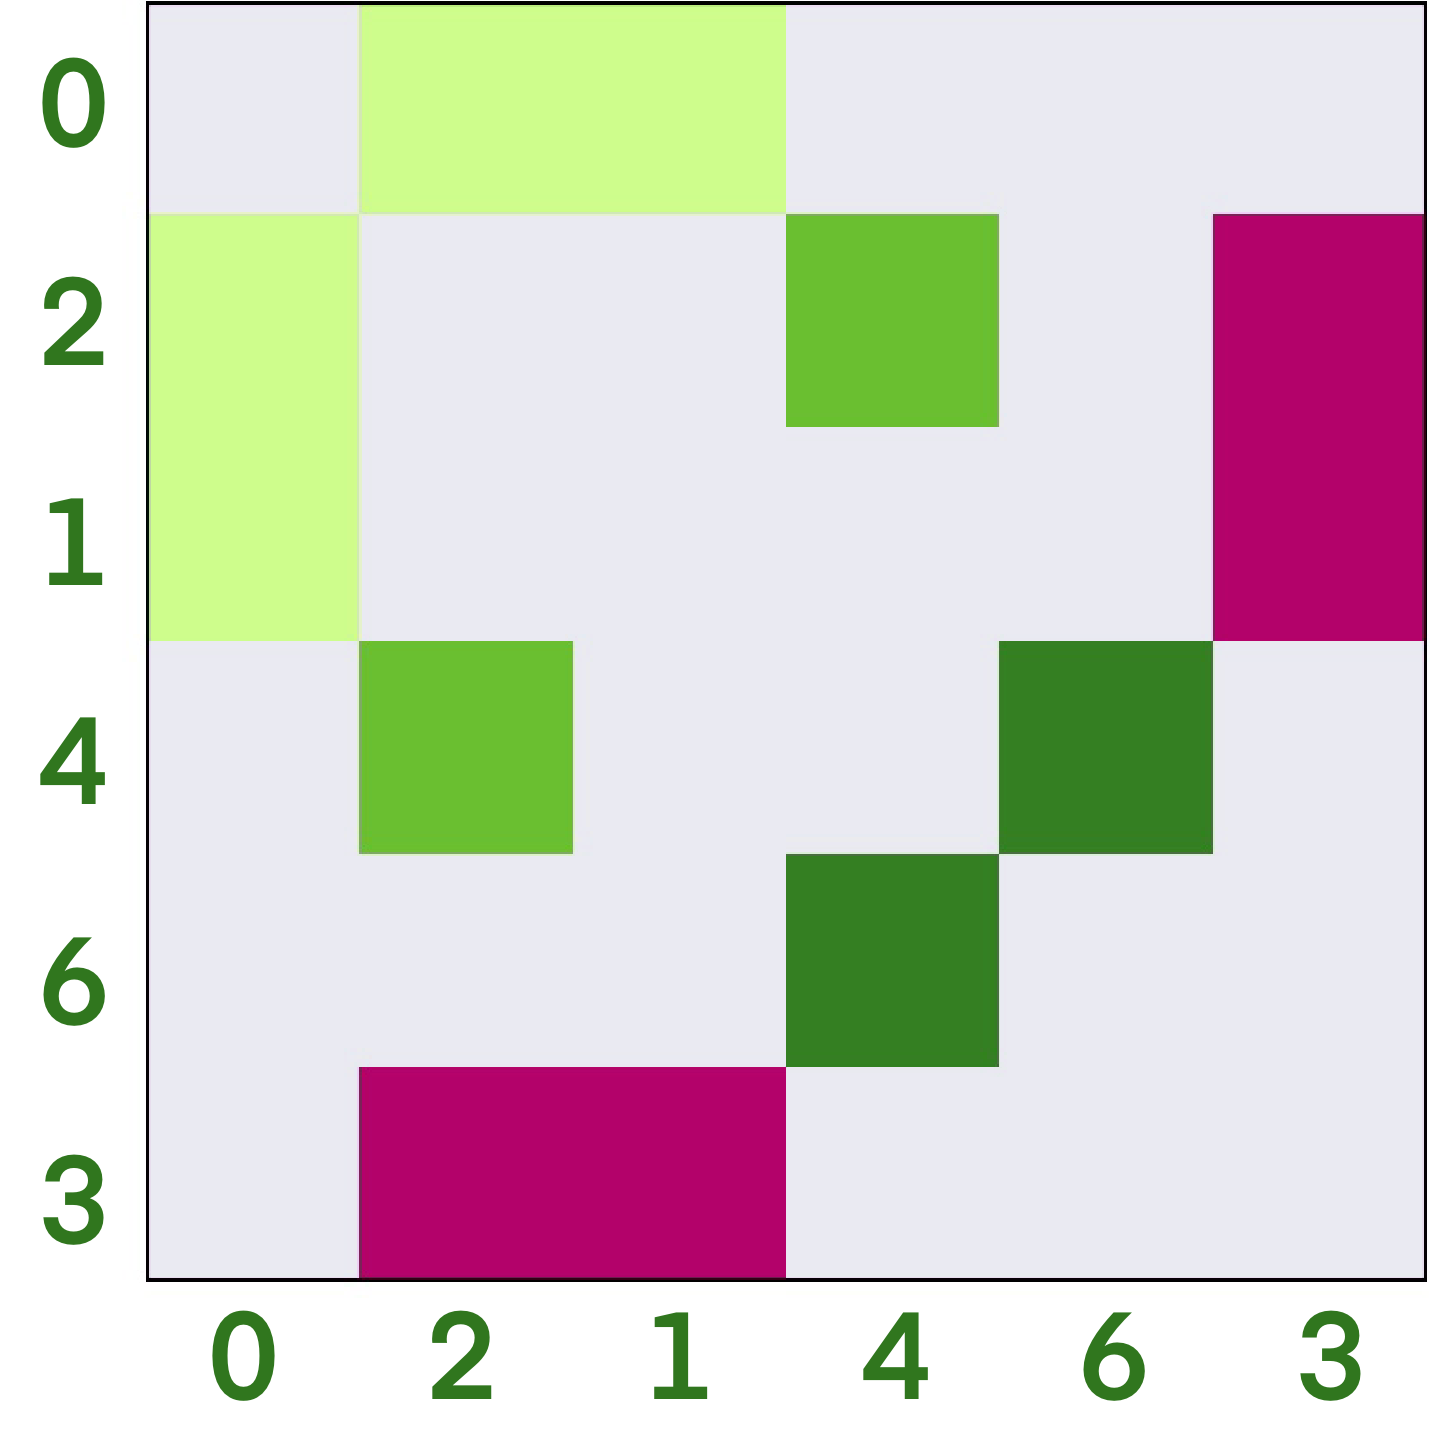
\includegraphics[width=\textwidth]{results/figures/dipole_yes_b.png}
        \caption{transition matrix for a 2D quantum dot when a magnetic field
            is applied.}
        \label{fig:transition_yes_b}
    \end{minipage}        
    \end{center}
\end{figure}

If we compute the frequency spectrum of the two systems
(\autoref{fig:transmission_spectrum_b_field}) we get a single line for the 
normal quantum dot. This is expected, as the quantum harmonic oscillator has 
the same energy difference between each level. However, when we apply a magnetic
field and shift the energies of the orbitals in the quantum dot, we see that we 
get two different energy transitions. This is revealed as two lines in the 
frequency spectrum in \autoref{fig:transmission_spectrum_b_field}. This is equivalent 
to a splitting in transmisstion spectra of quantum dot arrays under the effect 
of a magnetic field in experiments\cite{heitmann1993spectroscopy,meurer1992single}.

\begin{figure}
    \centering
    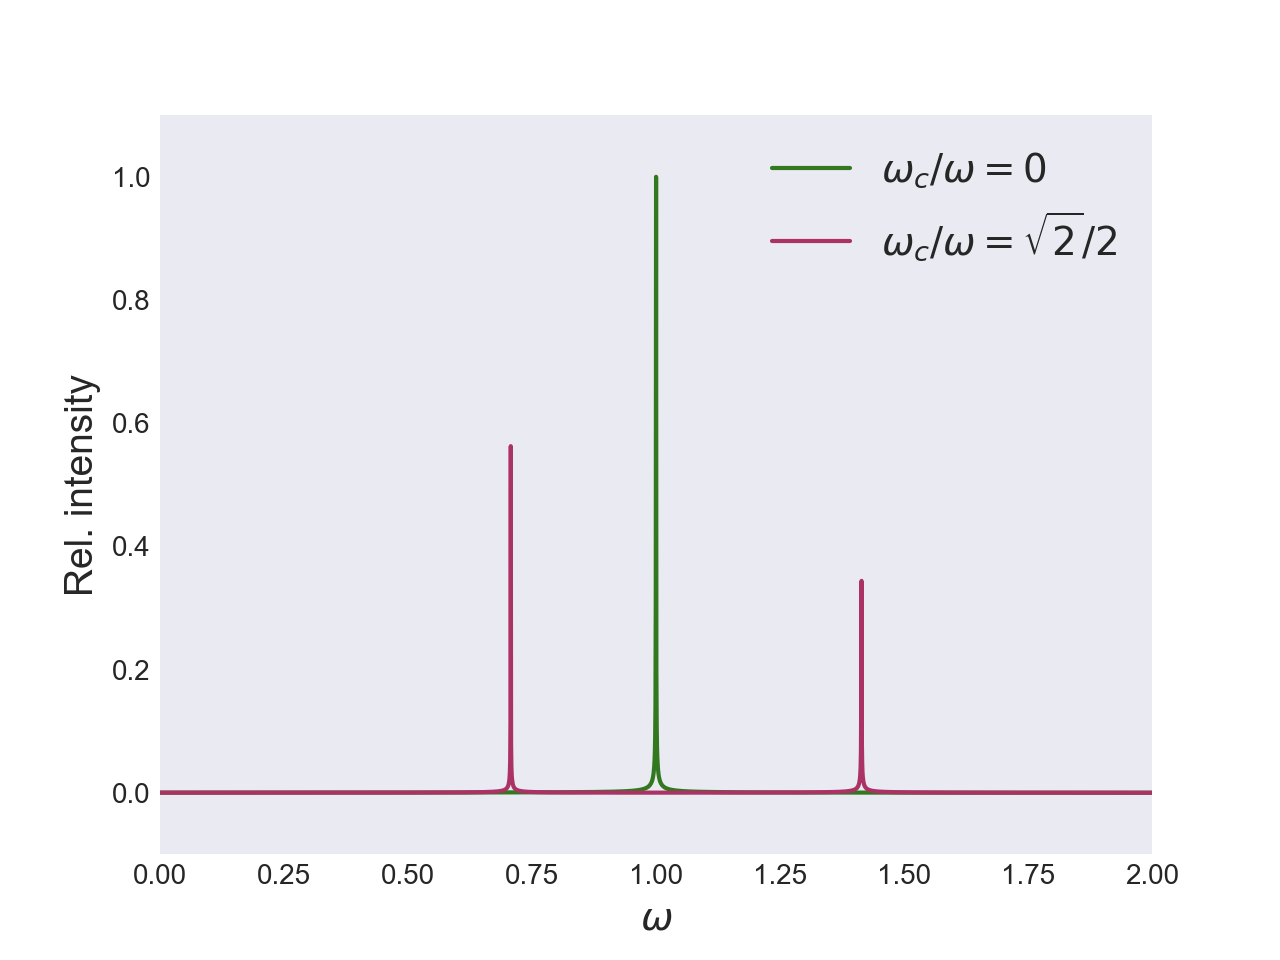
\includegraphics[width=0.75\textwidth]{results/figures/transmission_spectrum.png}
    \caption{Spectrum of a 2D quantum dot both with and without a magnetic field.}
    \label{fig:transmission_spectrum_b_field}
\end{figure}
